% !TEX root = cap06_standalone.tex
% Capítulo 5 del documento (archivo cap06). Resultados y análisis
% Estructura según índice de la Dra. Lárraga.
\graphicspath{{figures/}{../figures/}}

\chapter{Resultados y análisis}
\label{ch:resultados-analisis}

\begin{resumen}
Este capítulo presenta los resultados obtenidos de la aplicación del modelo WoE-AC para simular el crecimiento urbano de Querétaro. Se analiza la dinámica histórica observada (1984--2020), los resultados del análisis Weight of Evidence, la calibración del modelo, las simulaciones en cinco ventanas quinquenales desplazadas (2011--2016 a 2015--2020) y la evaluación cuantitativa mediante métricas espaciales (Accuracy, Precision, Recall, F1, Kappa, FoM). Finalmente, se realiza un análisis espacial del error para identificar las fuentes de discrepancia entre predicción y observación.
\end{resumen}

% ============================================================
\section{Dinámica observada del crecimiento urbano}
% ============================================================

Antes de evaluar el desempeño del modelo, es pertinente caracterizar el proceso que la simulación busca reproducir. Esta sección describe la evolución histórica de la huella urbana de Querétaro y los patrones espaciales de expansión identificados en la serie temporal 1984--2020.

\subsection{Evolución temporal 1984--2020}

Antes de presentar los resultados de la simulación conviene situarlos en el contexto histórico del crecimiento de Querétaro. Aquí hace falta una advertencia: la magnitud absoluta de la clase ``urbano'' que devuelve el clasificador no equivale a la mancha urbana real, porque arrastra también suelo desnudo y superficies áridas espectralmente parecidas (véase la nota metodológica al final de esta sección). Por eso, en vez de una tasa de crecimiento compuesta, que la serie clasificada no sostiene, la Tabla~\ref{tab:growth_periods} resume la fracción media de píxeles de esa clase en cuatro tramos de la serie.

\begin{table}[htbp]
\centering
\caption{Fracción media de píxeles clasificados como ``urbano'' por tramo de la serie 1984--2020. Las cifras provienen directamente de los mapas binarios y deben leerse como un indicador grueso de la dinámica, no como superficie construida.}
\label{tab:growth_periods}
\begin{tabular}{lll}
\toprule
\textbf{Período} & \textbf{Fracción media clasificada} & \textbf{Característica principal} \\
\midrule
1984--1995 & $\sim$43\% & Consolidación del centro urbano \\
1996--2005 & $\sim$44\% & Expansión hacia zonas industriales \\
2006--2015 & $\sim$45\% & Expansión dispersa (norte y este) \\
2016--2020 & $\sim$50\% & Consolidación periférica \\
\bottomrule
\end{tabular}
\end{table}

Sobre el conjunto de la serie, la fracción clasificada pasa de $44{,}42$\% en 1984 a $52{,}85$\% en 2020, un incremento neto de $8{,}4$ puntos porcentuales. La variabilidad interanual es alta: hay mínimos como $33{,}6$\% en 1992 y una desviación estándar cercana a $4$ puntos a lo largo del período. Un ajuste lineal de la fracción frente al año arroja una pendiente de apenas $0{,}15$ puntos por año, con $R^2 \approx 0{,}15$; es decir, la tendencia ascendente existe pero es débil y queda dominada por el ruido del clasificador. El único tramo que se separa con nitidez del resto es 2016--2020. Por eso no se reporta una tasa anual compuesta: la serie no la sostiene.

\begin{figure}[htbp]
\centering
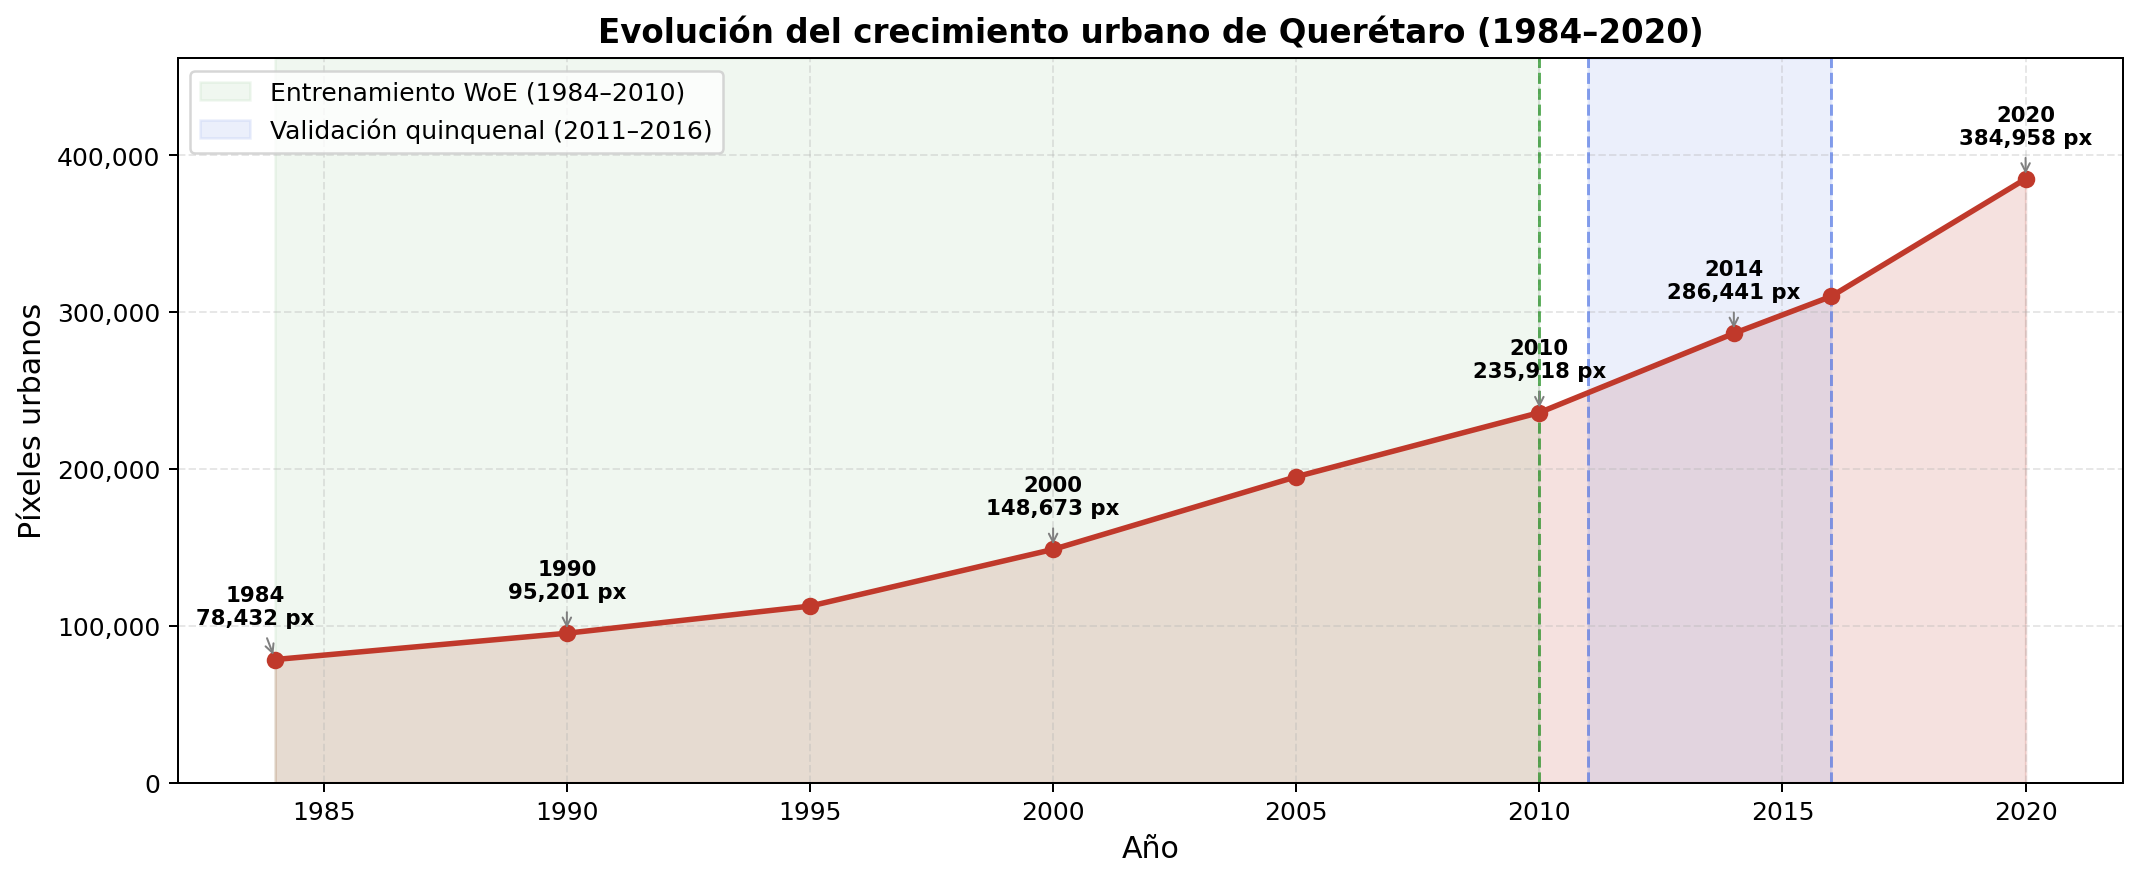
\includegraphics[width=0.9\textwidth]{figures/urban_growth_timeline.png}
\caption{Evolución de la fracción clasificada como ``urbano'' en Querétaro (1984--2020). Se observa una tendencia ascendente con fuerte variabilidad interanual, más marcada en el tramo final de la serie.}
\label{fig:urban_growth_timeline}
\end{figure}

La Figura~\ref{fig:urban_growth_timeline} resume esa serie.

\subsection{Patrones espaciales de expansión}

Los mapas binarios generados para cada año revelan tres patrones principales de expansión. El primero es el crecimiento contiguo por difusión, donde la expansión se produce principalmente desde los bordes de áreas urbanas existentes, siguiendo el mecanismo de contagio espacial que los autómatas celulares capturan de manera natural. El segundo corresponde al desarrollo periurbano a lo largo de corredores de transporte, visible en los ejes norte (autopista a San Luis Potosí) y oeste (autopista a Celaya). El tercero es el desarrollo industrial puntual: la instalación de parques industriales (Aeropuerto Industrial, Querétaro Aerospace) genera núcleos discontinuos en la periferia.

Los mapas binarios muestran crecimiento sostenido de la huella urbana a lo largo del período. Para los años de inicio de los experimentos de validación, los recuentos de píxeles urbanos extraídos directamente de los mapas clasificados son los siguientes: 2011: 2\,699\,088 px; 2012: 2\,140\,433 px; 2013: 2\,140\,627 px; 2014: 2\,469\,631 px; 2015: 2\,145\,356 px; 2020 (observado): 2\,864\,122 px. Estas cifras corresponden directamente a los valores \texttt{urban\_start} y \texttt{urban\_end\_observed} de los archivos de resultados de validación (\texttt{validation\_results.json}) y son los insumos directos del Autómata Celular.

\textbf{Nota metodológica sobre la clase ``urbano'':} El clasificador K-Means+SVM opera sobre características espectrales y de textura extraídas de las \textbf{capturas RGB} de la serie (Google Earth, imagen histórica). En la práctica, el clasificador aprende a separar dos agrupaciones espectrales: \textit{zonas con cubierta vegetal verde y densa} versus \textit{zonas sin cubierta vegetal verde}. Esta segunda clase agrupa el tejido urbano real (edificaciones, vialidades, concreto), pero también suelo desnudo agrícola en temporada seca y superficies áridas periféricas espectralmente similares a las urbanas. Por ello, los recuentos de píxeles de la clase ``urbano'' son considerablemente mayores que la mancha urbana real de Querétaro.

La validación del modelo se realiza en términos de \textit{consistencia interna}: dado un mapa binario clasificado en el año $t$ (con la definición descrita), el modelo predice qué píxeles habrán cambiado de clase en $t+5$. La calidad de esa predicción es lo que miden las métricas de la Sección~\ref{sec:evaluacion}. Este enfoque es válido mientras la definición de clase se aplique de forma consistente en todos los años de la serie.

% ============================================================
\section{Resultados del análisis Weight of Evidence}
% ============================================================

Esta sección presenta los resultados del cálculo de Weight of Evidence sobre las transiciones históricas observadas (1984--2010), incluyendo el poder predictivo de cada variable espacial cuantificado mediante el Information Value y la interpretación geográfica de los pesos obtenidos.

\subsection{Transiciones históricas identificadas}

El cálculo de Weight of Evidence se basó en el análisis de 26 períodos anuales consecutivos (1984--2010), identificando los píxeles que cambiaron de estado entre cada par de años, hasta acumular $8\,196\,264$ transiciones observadas. Las siete variables espaciales se promediaron sobre esos 26 períodos y el mapa promedio se contrastó con el conjunto acumulado de transiciones, según el procedimiento descrito en el Capítulo~\ref{ch:modelo-crecimiento-urbano}. Los pesos resultantes describen, por tanto, el régimen espacial medio del período de entrenamiento.

\subsection{Pesos por variable (Information Value)}

El modelo utiliza 7 variables espaciales cuya importancia predictiva se cuantifica mediante el Information Value (IV). La Tabla~\ref{tab:iv_weights} presenta los IV calculados sobre el conjunto de entrenamiento 1984--2010 y el peso normalizado que se deriva de ellos, que es el que pondera a cada variable en la probabilidad de transición.

\begin{table}[htbp]
\centering
\caption{\textit{Information Value} y pesos normalizados de las siete variables WoE, calculados sobre el período de entrenamiento (1984--2010).}
\label{tab:iv_weights}
\begin{tabular}{lcc}
\toprule
\textbf{Variable} & \textbf{IV} & \textbf{Peso normalizado} \\
\midrule
Distancia al área urbana (\texttt{distance\_urban}) & $3{,}2697$ & $0{,}2815$ \\
Densidad de vecindad $3\times3$ (\texttt{neighbor\_density\_3x3}) & $2{,}8973$ & $0{,}2495$ \\
Densidad de vecindad $5\times5$ (\texttt{neighbor\_density\_5x5}) & $1{,}6782$ & $0{,}1445$ \\
Densidad de vecindad $7\times7$ (\texttt{neighbor\_density\_7x7}) & $1{,}2396$ & $0{,}1067$ \\
Fragmentación local (\texttt{local\_fragmentation}) & $1{,}2331$ & $0{,}1062$ \\
Gradiente urbano (\texttt{urban\_gradient}) & $1{,}1568$ & $0{,}0996$ \\
Tamaño del \textit{cluster} más cercano (\texttt{nearest\_cluster\_size}) & $0{,}1388$ & $0{,}0120$ \\
\midrule
\textbf{Total} & $\mathbf{11{,}6135}$ & $\mathbf{1{,}000}$ \\
\bottomrule
\end{tabular}
\end{table}

El peso normalizado de cada variable es su IV dividido entre el IV total de las siete. El patrón muestra que la distancia al área urbana y las tres variables de densidad concentran $0{,}782$ del peso ($78{,}2$\%), lo que es coherente con un mecanismo de difusión espacial desde las áreas ya urbanizadas. La variable \texttt{nearest\_cluster\_size} recibe un peso muy bajo ($0{,}012$, con un IV de $0{,}139$), lo que sugiere que el tamaño del \textit{cluster} urbano más cercano aporta información marginal una vez controlada la distancia.

\subsection{Interpretación de los pesos WoE}

El patrón observado en los pesos es \textbf{coherente} con la teoría de difusión urbana, aunque no de forma monótona. Para las tres variables de densidad de vecindad, los pesos de los \textit{bins} 1--3 son negativos ($-5{,}58$ a $-0{,}40$ en el radio $3\times3$): corresponden a celdas con vecindad escasamente urbanizada y, en consecuencia, con menor probabilidad de transición que el promedio. Los \textit{bins} 4--8 son positivos y contienen la evidencia favorable a la transición, con un máximo de $+0{,}93$ ($3\times3$), $+0{,}87$ ($5\times5$) y $+0{,}80$ ($7\times7$) en $\rho \approx 0{,}37$--$0{,}55$. El punto de equilibrio (WoE $\approx 0$) se alcanza en $\rho \approx 0{,}10$--$0{,}15$, según el radio.

La relación es, por tanto, unimodal y no monótona. Pasado el máximo, la evidencia decae: el peso del radio $3\times3$ baja de $+0{,}93$ en $\rho \approx 0{,}37$--$0{,}55$ a $+0{,}21$ en el intervalo $\rho \approx 0{,}74$--$0{,}92$, que es el más alto que una celda candidata puede alcanzar. La lectura es directa y refuerza el mecanismo de difusión: la evidencia favorable se concentra en vecindades parcialmente urbanizadas, no en las que ya están próximas a la saturación, donde queda poco suelo disponible alrededor. El crecimiento ocurre en el frente urbano, no dentro de la mancha consolidada. La Figura~\ref{fig:woe_weights} resume la contribución de cada variable y la amplitud de sus pesos.

\subsubsection{Alcance de los bins extremos y de la jerarquía entre variables}
\label{ssec:alcance-iv}

Los pesos anteriores se estimaron sobre todas las celdas de la rejilla, sin restringir el muestreo a las celdas elegibles, es decir, a las que eran no urbanas en el año inicial. Conviene precisar el alcance de esa decisión, porque afecta a dos bins y a la lectura del \textit{Information Value}.

El efecto se concentra en dos intervalos. El \textit{bin} de distancia nula de \texttt{distance\_urban} agrupa las celdas que ya eran urbanas, y el \textit{bin} de densidad unitaria del radio $3\times3$ agrupa las de vecindad completamente urbanizada. Ninguno de los dos registra transiciones observadas, de modo que su peso ($-14{,}28$ y $-13{,}78$) queda determinado por el suavizado que evita la división por cero, no por los datos. Lo que ambos codifican es la restricción estructural de que una celda urbana no vuelve a urbanizarse, no un gradiente de evidencia espacial.

Ninguno de los dos pesos interviene en la simulación, y no por una precaución añadida sino por la propia construcción de las variables. El autómata evalúa como candidatas únicamente las celdas no urbanas. Una celda no urbana tiene distancia al frente urbano mayor o igual que uno, mientras que el \textit{bin} degenerado de \texttt{distance\_urban} cubre el intervalo $[0;\ 0{,}0385]$: es inalcanzable. Y la densidad de vecindad se calcula con una ventana $3\times3$ que incluye la celda central, de modo que si el centro es no urbano la densidad no puede exceder $8/9 \approx 0{,}889$, mientras que el \textit{bin} degenerado exige densidad exactamente unitaria: también es inalcanzable. La comprobación sobre las diez rejillas del período de validación confirma el argumento sin excepciones: de $28\,917\,357$ celdas candidatas, ninguna cae en ninguno de los dos \textit{bins}. El detalle está en \texttt{data/processed/woe\_bin\_reachability.json}.

Queda entonces acotado dónde sí influyen. Los IV de la Tabla~\ref{tab:iv_weights} superan con holgura el umbral de $0{,}50$ que la escala convencional de la Sección~\ref{ssec:information-value} marca como muy fuerte, y esa magnitud no debe leerse como capacidad predictiva excepcional, porque proviene en buena parte de esos dos \textit{bins}: en \texttt{distance\_urban} el degenerado aporta $2{,}786$ de sus $3{,}270$ de IV, un $85{,}2$\%, y en el radio $3\times3$, $1{,}617$ de $2{,}897$, un $55{,}8$\%. Las otras cinco variables no tienen \textit{bins} degenerados. Como el IV determina la ponderación $\omega_k$ de la ecuación~\ref{eq:woe_ponderado}, el efecto real es sobre el peso relativo entre variables: descontando esos \textit{bins}, la densidad de vecindad $5\times5$ pasaría al primer lugar ($1{,}678$) y \texttt{distance\_urban} caería al sexto ($0{,}484$).

De ahí se sigue qué afirmar y qué no. La ponderación de la Tabla~\ref{tab:iv_weights} concede a la distancia más influencia que la que le correspondería con los \textit{bins} descontados, y es la ponderación con la que se obtuvieron todos los resultados de este capítulo: se validó fuera de muestra en cinco ventanas que no intervinieron en su estimación, con los valores de FoM, Kappa e IoU ya reportados. Lo que se sostiene en cualquiera de las dos lecturas es que la señal que gobierna la simulación es la difusión por contigüidad, porque las cuatro variables de densidad y fragmentación conservan su posición relativa. Lo que no se sostiene sin esta salvedad es la primacía de la distancia sobre la densidad como jerarquía de capacidad discriminante. Restringir el muestreo a celdas elegibles depuraría la interpretación de los IV sin alterar la mecánica de la simulación, y por eso figura entre las extensiones del Capítulo~\ref{ch:conclusiones} y no entre las correcciones pendientes.

\begin{figure}[htbp]
\centering
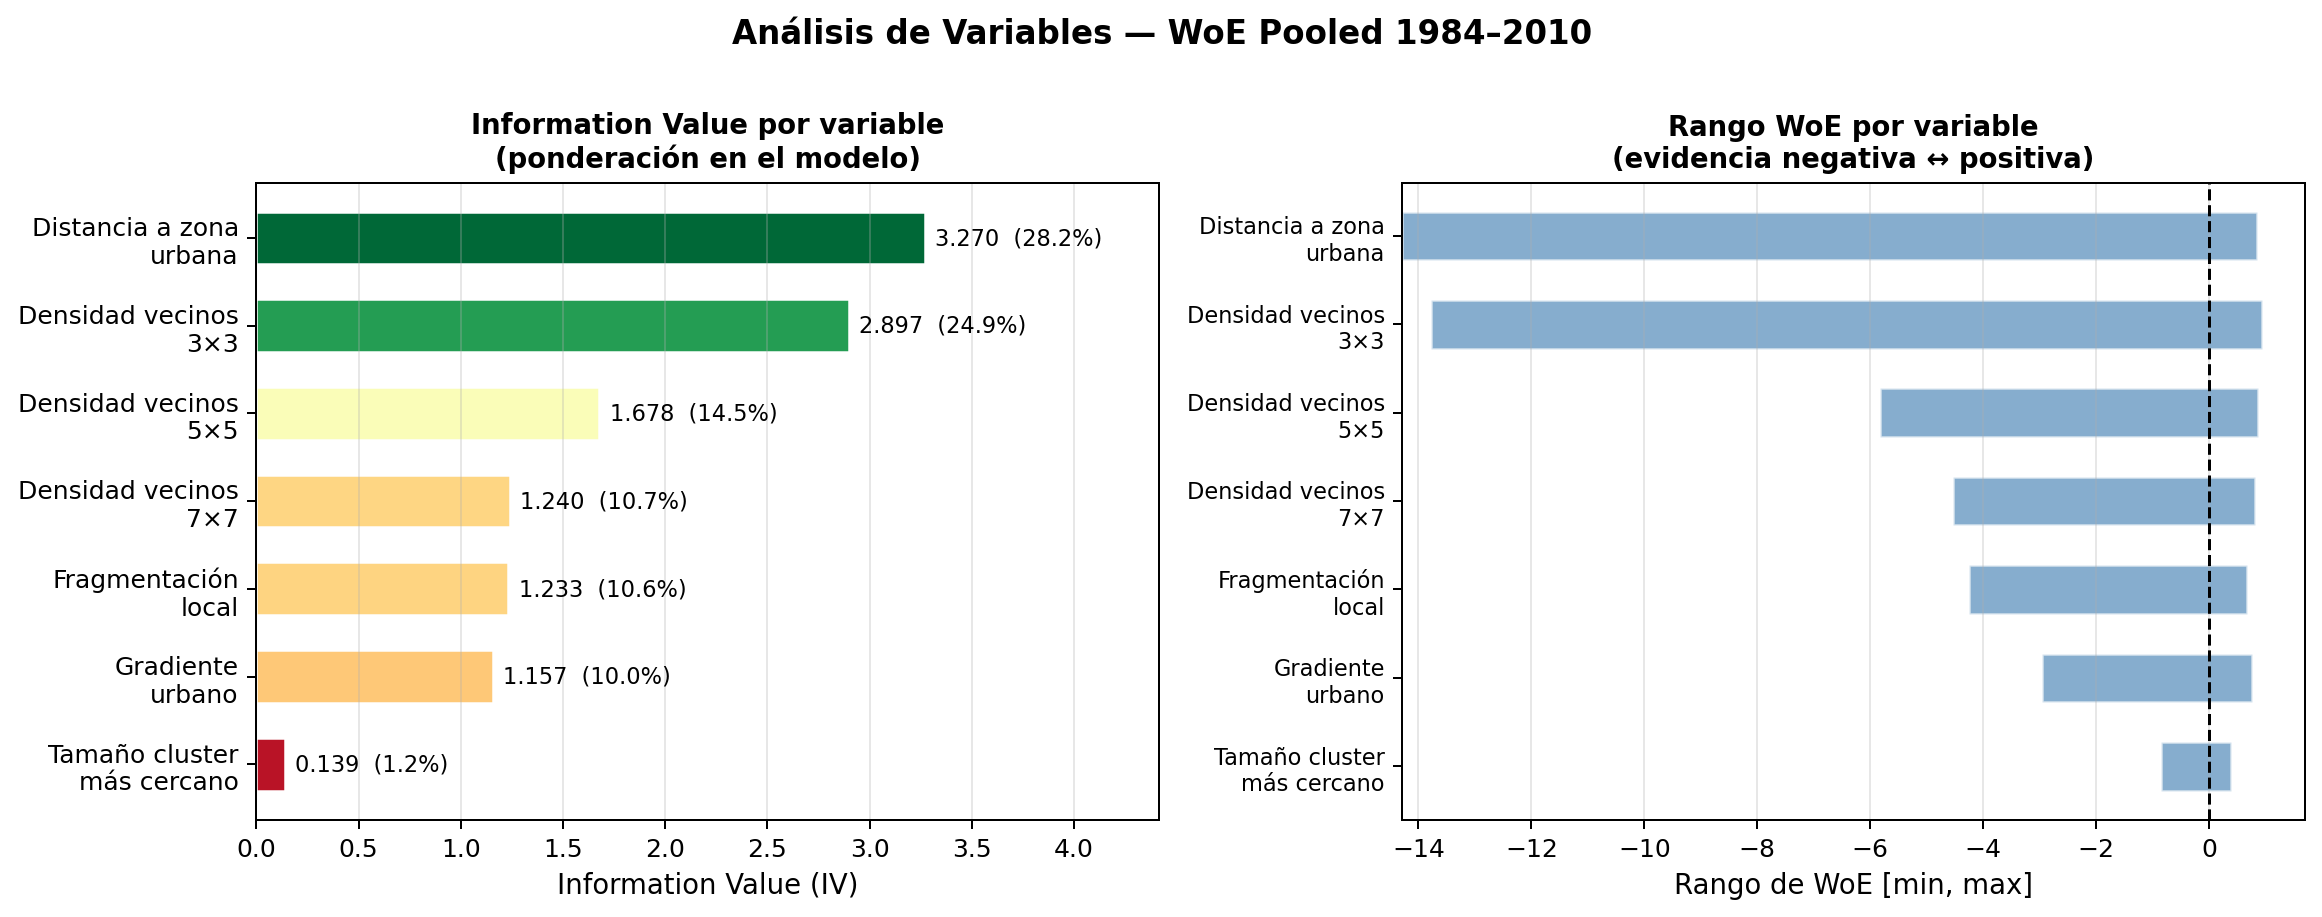
\includegraphics[width=0.7\textwidth]{figures/woe_weights.png}
\caption{\textit{Information Value} por variable (izquierda) y rango de pesos WoE por variable (derecha), calculados sobre el período de entrenamiento 1984--2010. La distancia al área urbana concentra el IV más alto ($3{,}270$, un $28{,}2$\% del total), por encima de la densidad de vecindad $3\times3$ ($2{,}897$, un $24{,}9$\%). El panel derecho muestra que ambas variables son también las de mayor amplitud entre evidencia negativa y positiva.}
\label{fig:woe_weights}
\end{figure}

% ============================================================
\section{Calibración del modelo}
% ============================================================

A partir de los pesos WoE derivados de los datos históricos, esta sección describe la configuración final del Autómata Celular y el proceso de calibración sistemática de sus parámetros mediante búsqueda en cuadrícula (\textit{grid search}). El marco metodológico que justifica esta elección se discute en el Capítulo~\ref{ch:modelo-crecimiento-urbano} (Sección~\ref{sec:definicion-modelo}).

\subsection{Configuración del autómata celular}

El Autómata Celular se configuró con los parámetros especificados en la Tabla~\ref{tab:ac_final_config}, resultado de la calibración sobre el conjunto de entrenamiento (1984--2010).

\begin{table}[htbp]
\centering
\caption{Configuración final del Autómata Celular WoE-AC.}
\label{tab:ac_final_config}
\begin{tabularx}{\textwidth}{@{}>{\bfseries}p{0.30\textwidth}X@{}}
\toprule
Parámetro & Valor \\
\midrule
Espacio celular & $1\,792 \times 3\,024$ píxeles. \\
Estados & $\{0:\text{no-urbano},\ 1:\text{urbano}\}$. \\
Vecindario & Moore (8 vecinos, radio $=1$). \\
Variables WoE & Siete variables espaciales: distancia al área urbana, densidades de vecindad $3\times3$, $5\times5$ y $7\times7$, fragmentación local, gradiente urbano y tamaño del \textit{cluster} más cercano. \\
Ponderación de variables & Proporcional al \textit{Information Value} (IV) normalizado. \\
Umbral de urbanización & $\theta = 0{,}75$ (calibrado sobre la probabilidad combinada). \\
Peso de vecindad & $\alpha = 0{,}50$. \\
Paso temporal & 1 año. \\
Períodos de simulación & 5 iteraciones por experimento. \\
\bottomrule
\end{tabularx}
\end{table}

\subsection{Proceso de calibración}

La calibración se centró en el umbral de urbanización ($\theta$) y en la ponderación de las siete variables WoE, y se realizó sobre el período de entrenamiento (1984--2010). El umbral final $\theta = 0{,}75$ se adoptó porque los valores ensayados en la exploración inicial ($\approx 0{,}40$--$0{,}60$) producían una sobre-predicción excesiva del crecimiento urbano: la mejor configuración de ese rango, con $\theta = 0{,}400$, simuló $2\,203\,593$ transiciones frente a las $391\,095$ observadas y alcanzó un FoM de $0{,}172$, muy por debajo del que se obtiene con el umbral adoptado. Ya en la fase de validación, y como resultado y no como criterio de ajuste, esa configuración reduce la sobre-predicción y mantiene el Recall por encima de $0{,}91$ en las cinco ventanas evaluadas. La ponderación de las siete variables WoE se hizo proporcional al \textit{Information Value} (IV) de cada variable, calculado sobre el conjunto de entrenamiento (1984--2010). La configuración resultante (umbral, peso de vecindad y ponderación por IV) queda documentada en el repositorio, junto con los scripts que reproducen el barrido. El detalle de rutas se recoge en el Apéndice~\ref{ap:arquitectura}.

La probabilidad de urbanización para la celda $(i,j)$ en el paso $t$ es la misma regla de transición definida en el Capítulo~\ref{ch:modelo-crecimiento-urbano} (ecuación~\ref{eq:transicion}): el campo WoE, suma de las siete evidencias ponderadas por su \textit{Information Value} normalizado, se transforma con la sigmoide y se le suma después la influencia del vecindario, acotando el resultado a $[0,1]$:
\begin{equation}
P_{\text{trans}}(i,j,t) = \min\!\left(1,\; \sigma\!\Big(\sum_{k=1}^{7} \frac{IV_k}{\sum_{l} IV_l}\, \cdot \,\text{WoE}_k(i,j,t)\Big) \;+\; \alpha \cdot I_{\text{neigh}}(i,j,t)\right),
\end{equation}
donde $\sigma(\cdot)$ es la función sigmoide; $IV_k$, el \textit{Information Value} de la $k$-ésima variable; $\text{WoE}_k(i,j,t)$, el valor de evidencia en la celda; $\alpha = 0{,}50$, el peso de vecindad; e $I_{\text{neigh}}(i,j,t) \in [0,1]$, la fracción de vecinos urbanos en la vecindad de Moore. Una celda se urbaniza cuando $P_{\text{trans}}$ supera el umbral $\theta = 0{,}75$ y un sorteo aleatorio lo confirma.

% ============================================================
\section{Simulación del crecimiento urbano}
% ============================================================

Esta sección describe el protocolo de validación quinquenal múltiple implementado para evaluar el desempeño del modelo en régimen de \textit{hold-out} respecto del período de entrenamiento, y presenta los resultados individuales de las simulaciones en cada uno de los cinco períodos evaluados.

\subsection{Protocolo de validación quinquenal múltiple}

Para evaluar el modelo de forma independiente del entrenamiento, se adoptó un esquema de \textbf{validación quinquenal múltiple}: el WoE se entrenó exclusivamente con datos del período 1984--2010 y, con esos pesos, el Autómata Celular se simuló en cinco ventanas temporales solapadas de cinco años, con años de inicio sucesivos (2011, 2012, 2013, 2014 y 2015). El diseño separa entrenamiento y prueba: ningún dato del período de validación interviene en el entrenamiento (\textit{hold-out} temporal) y permite evaluar la estabilidad del modelo bajo distintas condiciones de partida. La Tabla~\ref{tab:simulation_config} reúne la configuración con la que se ejecutaron las cinco simulaciones.

\begin{table}[htbp]
\centering
\caption{Configuración del experimento de validación quinquenal múltiple.}
\label{tab:simulation_config}
\begin{tabular}{ll}
\toprule
\textbf{Parámetro} & \textbf{Valor} \\
\midrule
WoE entrenado con & 1984--2010 (26 transiciones anuales agregadas por \textit{pooling}) \\
Umbral de urbanización & $\theta = 0{,}75$ \\
Peso de vecindad & $\alpha = 0{,}50$ \\
Pasos por validación & 5 iteraciones (1 año por paso) \\
Períodos evaluados & 2011--2016, 2012--2017, 2013--2018, 2014--2019 y 2015--2020 \\
\bottomrule
\end{tabular}
\end{table}

% ============================================================
\section{Evaluación del modelo}
\label{sec:evaluacion}
% ============================================================

A continuación se presentan las métricas de evaluación cuantitativa del modelo en los cinco períodos quinquenales y se contextualizan los resultados frente a valores de referencia reportados en la literatura internacional.

\subsection{Resumen comparativo -- cinco períodos quinquenales}

La Tabla~\ref{tab:metrics_all_periods} resume las métricas obtenidas en los cinco períodos evaluados. El \textbf{FoM promedio es de $0{,}317$} (equivalente a $31{,}7\%$ en escala porcentual), calculado conforme a la Ecuación~\ref{eq:fom_formula} del marco teórico. Esta magnitud se sitúa en una \textbf{banda intermedia} del espectro empírico documentado por \textcite{pontius2008comparing}: por encima del subconjunto de aplicaciones con FoM inferior a $0{,}15$ y muy por debajo del único caso que supera $0{,}50$ en esa muestra multi-sitio (Capítulo~\ref{ch:estado-del-arte}). El Kappa promedio de $0{,}445$ corresponde a un acuerdo moderado según la escala de \textcite{LandisKoch1977}, en la parte baja de ese rango ($0{,}41$--$0{,}60$). El Recall alto ($>0{,}91$ en todos los períodos) indica que el modelo captura la mayor parte de la urbanización observada, bajo la misma definición operativa de la clase urbana, aunque con sobre-predicción sistemática de la magnitud del crecimiento.

\begin{table}[htbp]
\centering
\caption{Métricas de validación en las cinco ventanas quinquenales (WoE-AC, umbral $\theta=0{,}75$).}
\label{tab:metrics_all_periods}
\small
\setlength{\tabcolsep}{3.5pt}
\resizebox{\linewidth}{!}{%
\begin{tabular}{lrrrrrrr}
\toprule
\textbf{Período} & \textbf{Acc} & \textbf{IoU} & \textbf{Prec} & \textbf{Recall} & \textbf{F1} & \textbf{$\kappa$} & \textbf{FoM} \\
\midrule
2011--2016 & $0{,}665$ & $0{,}581$ & $0{,}590$ & $0{,}975$ & $0{,}735$ & $0{,}349$ & $0{,}222$ \\
2012--2017 & $0{,}750$ & $0{,}652$ & $0{,}688$ & $0{,}925$ & $0{,}789$ & $0{,}499$ & $0{,}345$ \\
2013--2018 & $0{,}744$ & $0{,}648$ & $0{,}689$ & $0{,}917$ & $0{,}787$ & $0{,}482$ & $0{,}355$ \\
2014--2019 & $0{,}697$ & $0{,}614$ & $0{,}628$ & $0{,}965$ & $0{,}761$ & $0{,}396$ & $0{,}287$ \\
2015--2020 & $0{,}755$ & $0{,}669$ & $0{,}701$ & $0{,}936$ & $0{,}802$ & $0{,}498$ & $0{,}378$ \\
\midrule
\textbf{Promedio} & $\mathbf{0{,}722}$ & $\mathbf{0{,}633}$ & $\mathbf{0{,}659}$ & $\mathbf{0{,}944}$ & $\mathbf{0{,}775}$ & $\mathbf{0{,}445}$ & $\mathbf{0{,}317}$ \\
\bottomrule
\end{tabular}%
}
\end{table}

La variación entre períodos refleja diferencias en la dinámica observada. El período 2011--2016 muestra el FoM más bajo ($0{,}222$): el área urbana clasificada en 2016 \textit{decreció} levemente respecto a 2011, una anomalía atribuible a la variabilidad de la clasificación binaria RGB año a año, más que a una contracción urbana real. Los períodos 2012--2017, 2013--2018 y 2015--2020, en los que el crecimiento neto observado es positivo, exhiben FoM entre $0{,}345$ y $0{,}378$, con mayor concordancia entre el modelo y los mapas observados. La Tabla~\ref{tab:literature_comparison} sitúa estos valores frente al espectro documentado en la literatura.

\begin{table}[htbp]
\centering
\caption{Posicionamiento del modelo WoE-AC en el espectro empírico de Figure of Merit (FoM) documentado en la literatura LUCC. La comparación es cualitativa: los sitios, las definiciones temáticas de las clases y los horizontes temporales difieren entre estudios.}
\label{tab:literature_comparison}
\begin{tabularx}{\textwidth}{@{}>{\raggedright\arraybackslash}p{4.6cm} >{\raggedright\arraybackslash}p{2.8cm} X@{}}
\toprule
\textbf{Referencia} & \textbf{Método} & \textbf{FoM reportado / observado} \\
\midrule
Estudio comparativo multi-sitio \parencite{pontius2008comparing} & Trece aplicaciones de nueve modelos & Espectro empírico amplio: seis aplicaciones con FoM inferior a $0{,}15$ y una sola por encima de $0{,}50$; el FoM puede variar entre $0$ y $1$. \\
GSA-CA en Urumqi \parencite{Tang2024} & AC con búsqueda gravitacional & FoM = $0{,}430$ en calibración y $0{,}376$ en validación; contexto árido con \textit{drivers} físicos explícitos. \\
\textbf{Este trabajo (ZMQ, promedio cinco ventanas)} & \textbf{WoE-AC con \textit{grid search}} & \textbf{FoM promedio} = $\mathbf{0{,}317}$ (i.e., $\mathbf{31{,}7\%}$); \textbf{Kappa promedio} = $\mathbf{0{,}445}$. \\
\bottomrule
\end{tabularx}
\end{table}

Comparado con el estudio de \textcite{Tang2024} sobre Urumqi, presentado en el Capítulo~\ref{ch:estado-del-arte}, donde el aprovechamiento explícito de \textit{drivers} físicos asociados a la aridez eleva el FoM por encima de $0{,}37$, el modelo WoE-AC propuesto queda por debajo, lo que es coherente con el hecho de que en este trabajo se emplean exclusivamente variables derivadas del propio mapa binario, sin incorporar restricciones topográficas, socioeconómicas ni de infraestructura.

La Figura~\ref{fig:metricas-quinquenales} presenta esas mismas cifras en forma gráfica y admite dos lecturas que la tabla no hace evidentes. La primera es que las tres métricas coinciden en señalar las dos ventanas de menor desempeño, $2011$--$2016$ y $2014$--$2019$, que son también las de menor crecimiento neto observado; entre las tres restantes el orden cambia según la métrica que se privilegie, de modo que la jerarquía fina entre ellas no es robusta. La segunda es que la dispersión entre ventanas depende de la métrica: el FoM varía en un factor de $1{,}70$ entre el valor mínimo y el máximo, el Kappa en $1{,}43$ y el IoU en $1{,}15$. La razón está en el alcance de cada una. El IoU se calcula sobre la clase urbana completa e incorpora las celdas que ya eran urbanas al inicio del período, mientras que el FoM excluye por construcción el acierto sobre la permanencia y contabiliza solo celdas en transición (ecuación~\ref{eq:fom_formula}). El FoM es, por tanto, la métrica que discrimina con mayor amplitud entre ventanas, y es la que se privilegia al situar el modelo frente a la literatura.

\begin{figure}[htbp]
  \centering
  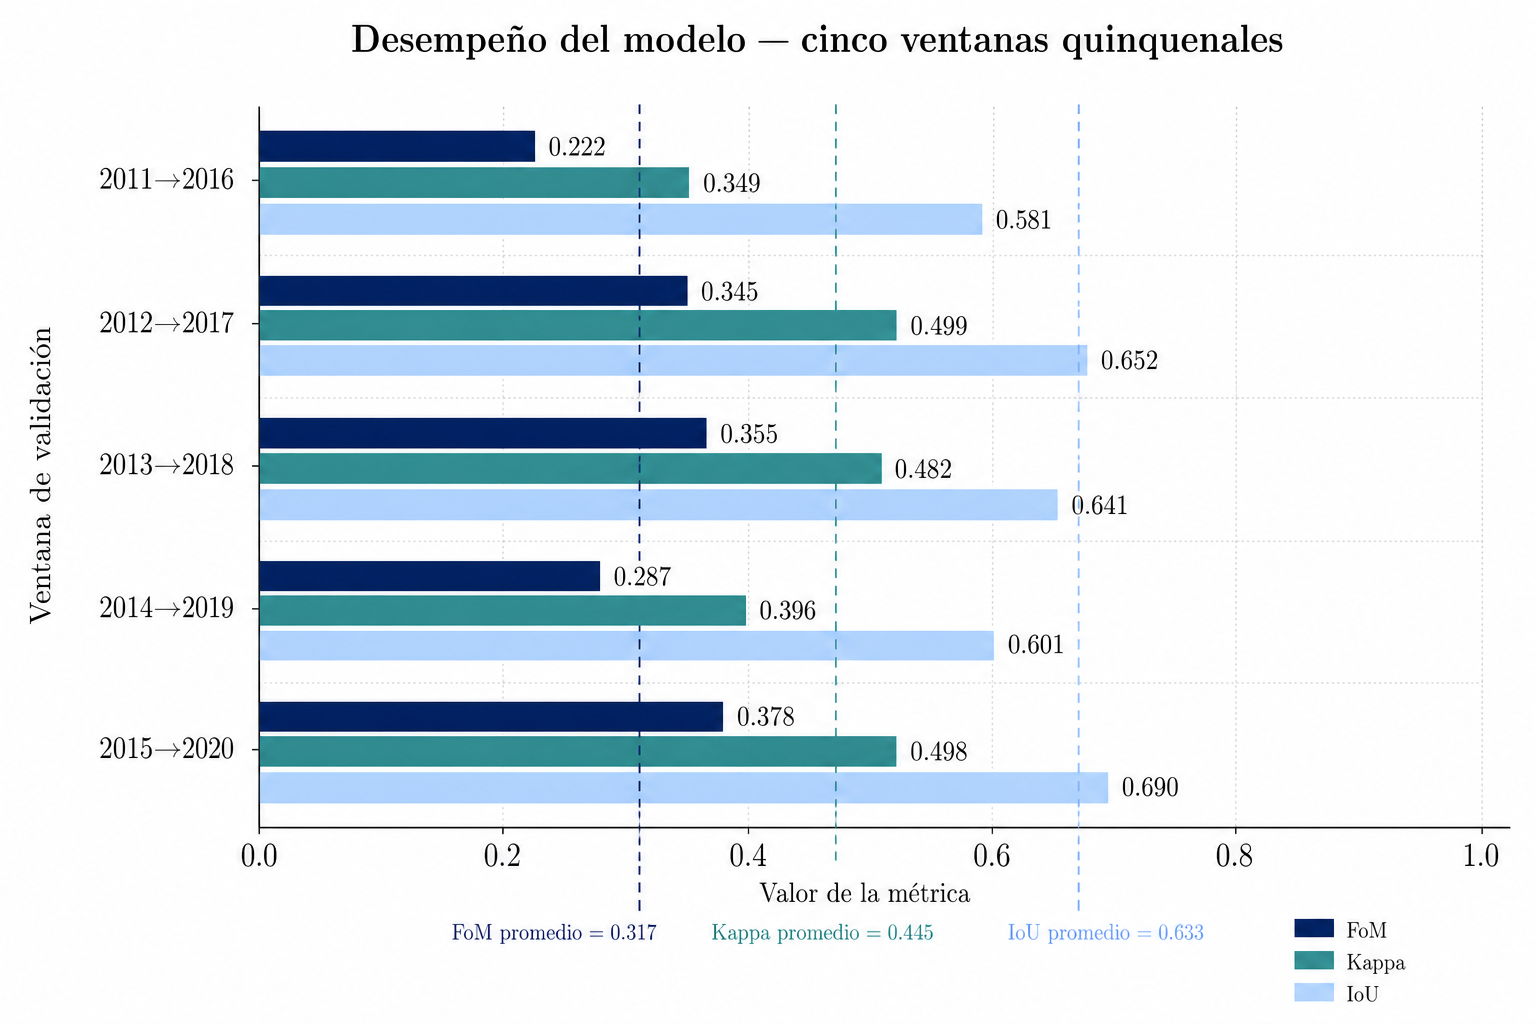
\includegraphics[width=0.92\linewidth]{F11_metricas_quinquenales_ai}
  \caption{Desempeño comparado del modelo WoE-AC en las cinco ventanas quinquenales. Las líneas verticales punteadas señalan el promedio de cada métrica: FoM $=0{,}317$, Kappa $=0{,}445$, IoU $=0{,}633$. El FoM más bajo coincide con la única ventana cuyo crecimiento neto observado es negativo. \textit{Figura elaborada con IA generativa a partir de los resultados de validación propios de la Tabla~\ref{tab:metrics_all_periods}.}}
  \label{fig:metricas-quinquenales}
\end{figure}


% ---- Períodos individuales ----
\clearpage
\subsection{Período 2011--2016}

La Tabla~\ref{tab:metrics_2011_2016} reúne las métricas de esta ventana y la Figura~\ref{fig:summary_2011_2016} compara el mapa observado con el predicho. Es el período con el FoM más bajo de la serie ($0{,}222$), por la razón ya anticipada: el área urbana clasificada en 2016 quedó por debajo de la de 2011.

\begin{table}[H]
\centering
\caption{Métricas de validación del período 2011$\rightarrow$2016. \textit{B} (hits del FoM) es el subconjunto de \textit{TP} que corresponde a transiciones a urbano observadas y predichas simultáneamente; los píxeles permanentes ya urbanizados quedan incluidos en \textit{TP} pero no en \textit{B} (véase Ec.~\ref{eq:fom_formula}).}
\label{tab:metrics_2011_2016}
\small
\begin{tabular}{lrlr}
\toprule
\multicolumn{2}{c}{\textbf{Métricas de píxel}} & \multicolumn{2}{c}{\textbf{Figure of Merit}} \\
\midrule
Accuracy  & $0{,}665$ & FoM                  & \textbf{$0{,}222$} \\
IoU       & $0{,}581$ & Hits ($B$)           & $361\,614$ \\
Precision & $0{,}590$ & Falsas alarmas ($A$) & $1\,203\,567$ \\
Recall    & $0{,}975$ & Omisiones ($C$)      & $64\,208$ \\
F1        & $0{,}735$ & TP / FP / FN         & $2\,514\,806$ / $1\,749\,463$ / $64\,208$ \\
$\kappa$  & $0{,}349$ & Crec.\ obs.\ / pred.\ & $-4{,}4\%$ / $+58{,}0\%$ \\
\bottomrule
\end{tabular}
\end{table}

\begin{figure}[H]
\centering
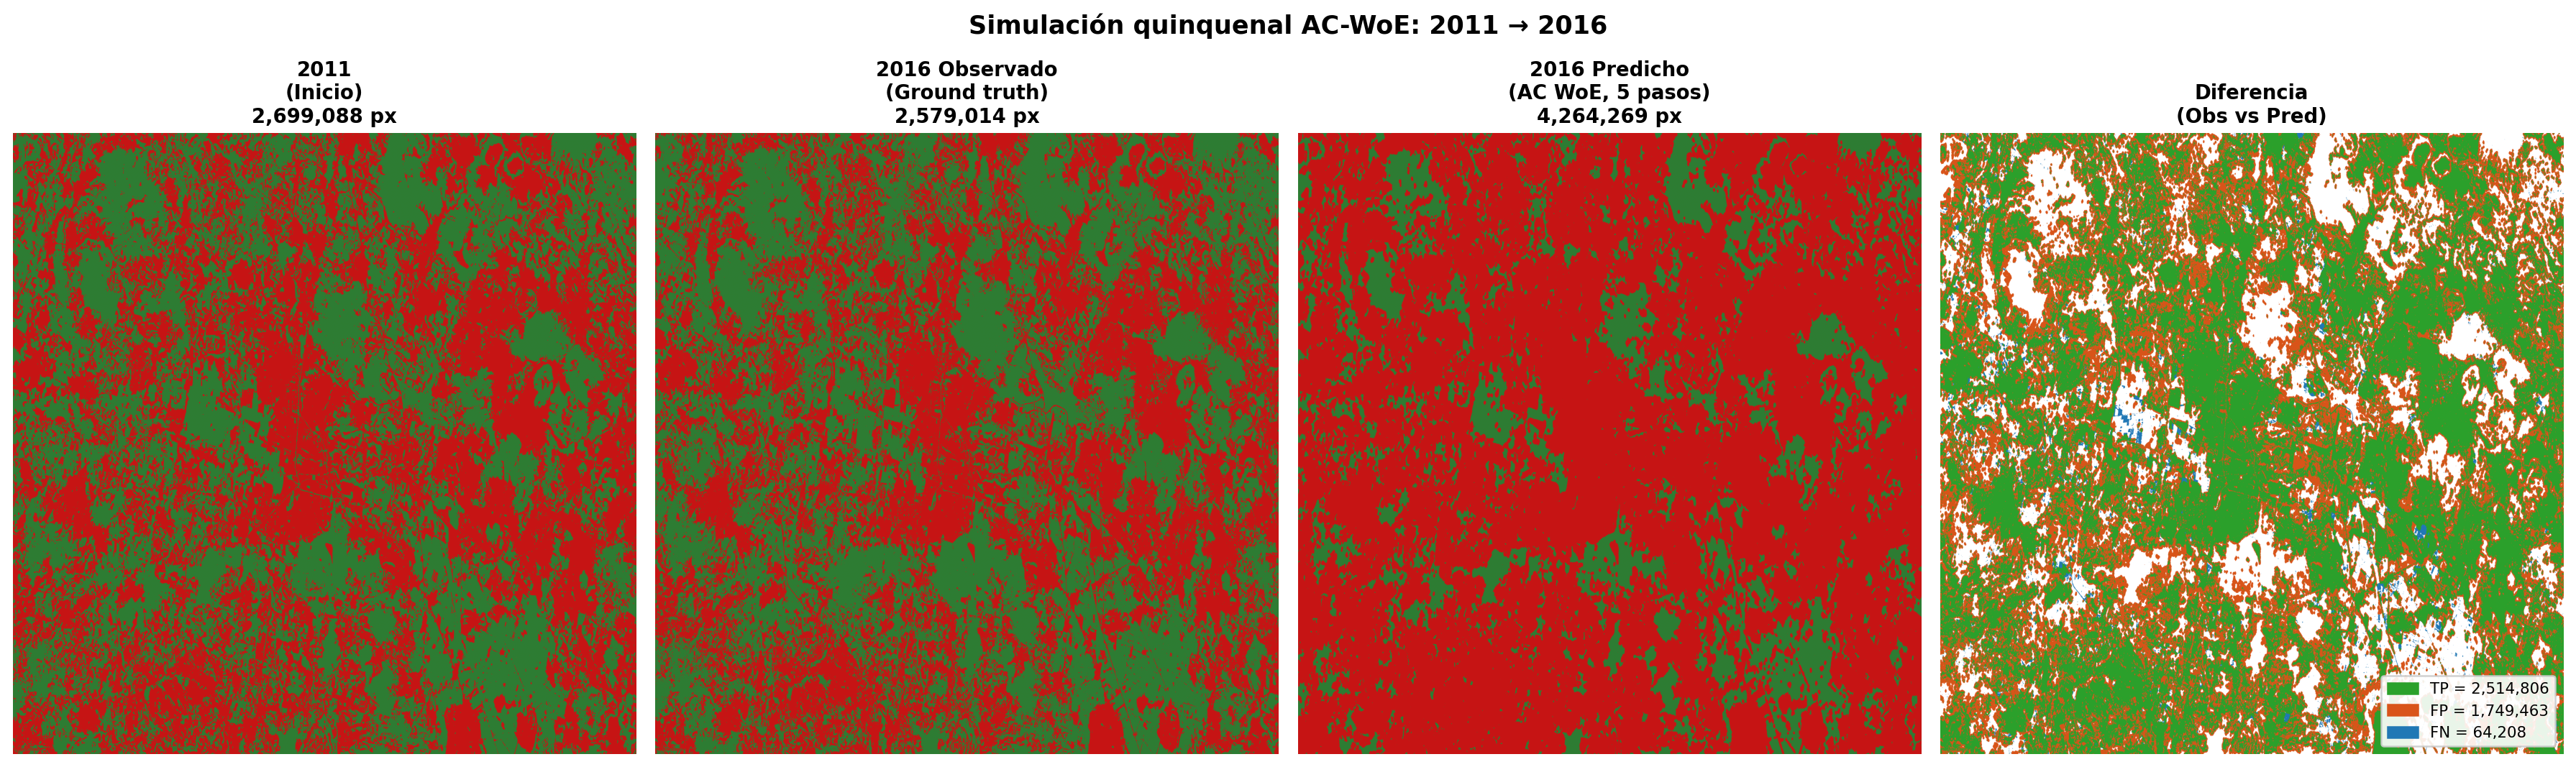
\includegraphics[width=\textwidth]{figures/summary_2011_to_2016.png}
\caption{Validación quinquenal 2011--2016. De izquierda a derecha: estado inicial (2011), mapa observado 2016 (\textit{ground truth}), mapa predicho 2016 y diferencia (verde=TP, naranja=FP, azul=FN). FoM $=0{,}222$; la anomalía se debe a que el área urbana observada disminuyó levemente por variabilidad en la clasificación binaria RGB año a año.}
\label{fig:summary_2011_2016}
\end{figure}

\clearpage
\subsection{Período 2012--2017}

En esta ventana el desempeño mejora respecto a la anterior. La Tabla~\ref{tab:metrics_2012_2017} detalla las métricas y la Figura~\ref{fig:summary_2012_2017} ilustra el resultado espacial, con un FoM de $0{,}345$ sobre un crecimiento observado positivo.

\begin{table}[H]
\centering
\caption{Métricas de validación del período 2012$\rightarrow$2017.}
\label{tab:metrics_2012_2017}
\small
\begin{tabular}{lrlr}
\toprule
\multicolumn{2}{c}{\textbf{Métricas de píxel}} & \multicolumn{2}{c}{\textbf{Figure of Merit}} \\
\midrule
Accuracy  & $0{,}750$ & FoM                  & \textbf{$0{,}345$} \\
IoU       & $0{,}652$ & Hits ($B$)           & $602\,889$ \\
Precision & $0{,}688$ & Falsas alarmas ($A$) & $937\,345$ \\
Recall    & $0{,}925$ & Omisiones ($C$)      & $205\,308$ \\
F1        & $0{,}789$ & TP / FP / FN         & $2\,532\,942$ / $1\,147\,725$ / $205\,308$ \\
$\kappa$  & $0{,}499$ & Crec.\ obs.\ / pred.\ & $+27{,}9\%$ / $+72{,}0\%$ \\
\bottomrule
\end{tabular}
\end{table}

\begin{figure}[H]
\centering
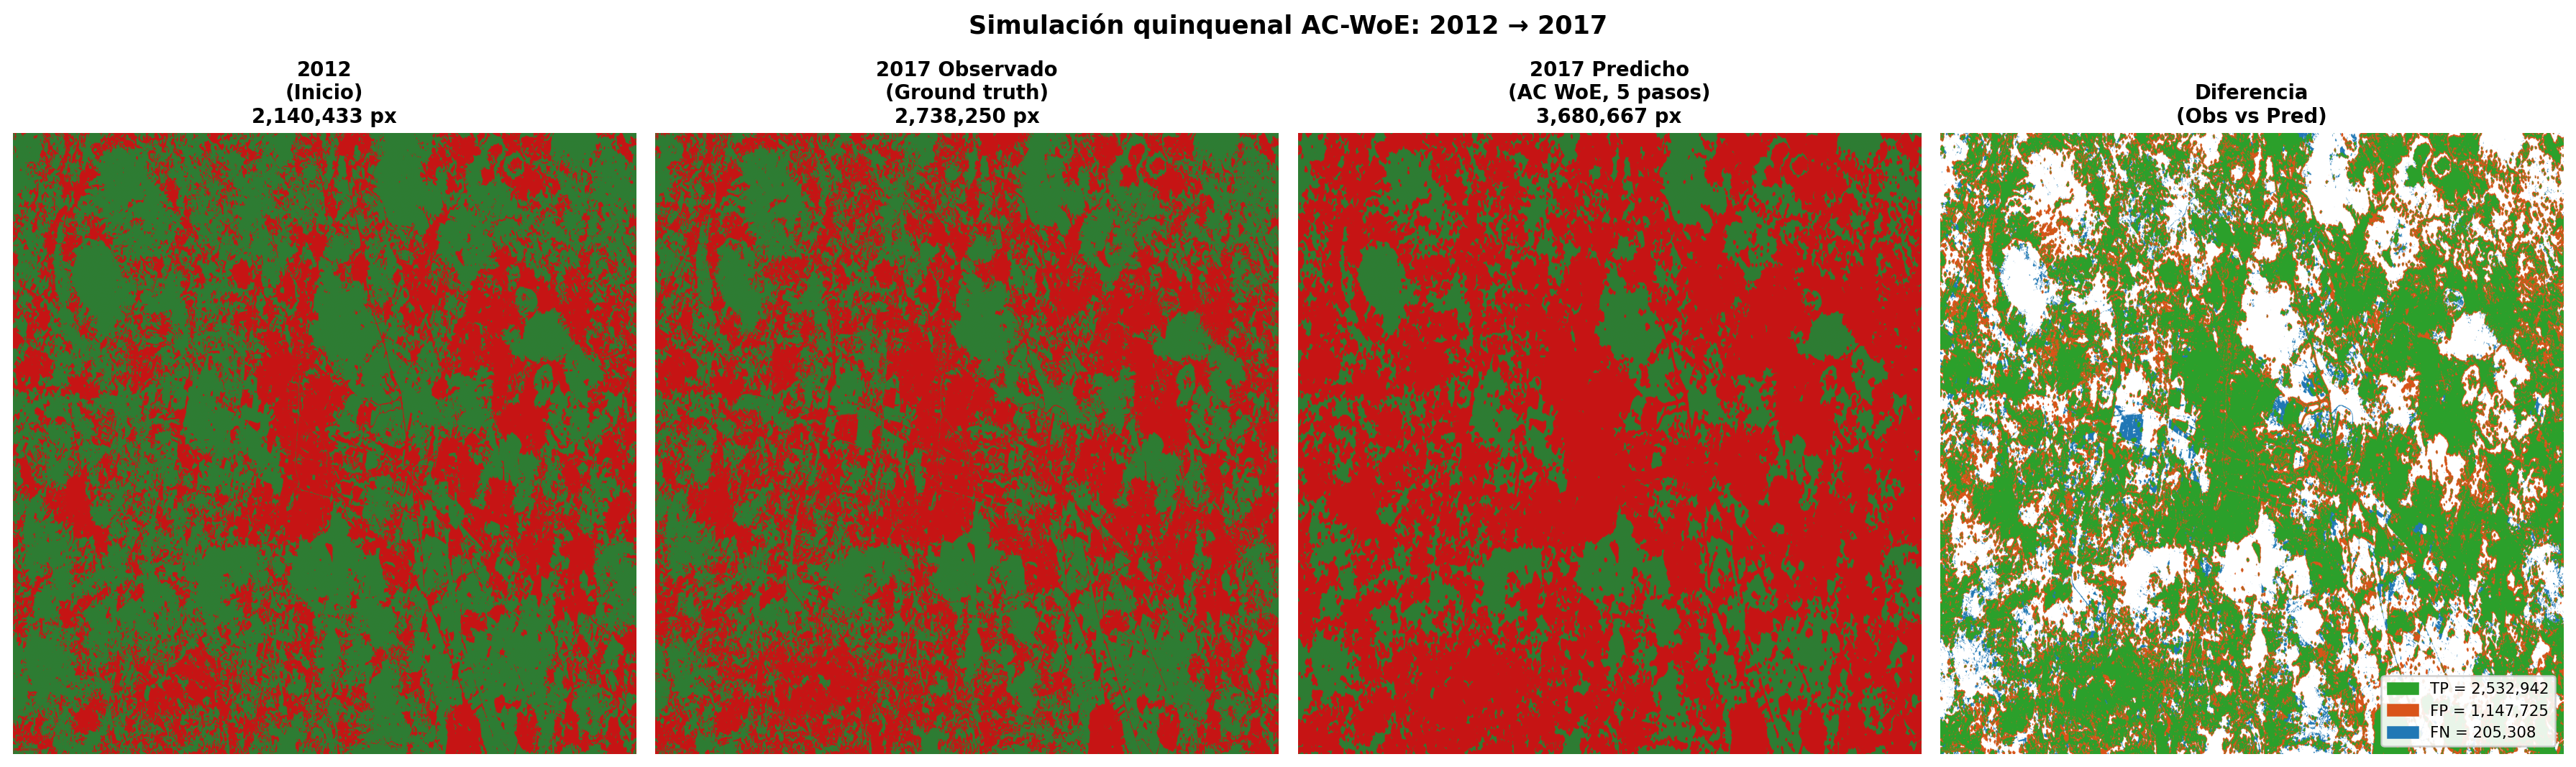
\includegraphics[width=\textwidth]{figures/summary_2012_to_2017.png}
\caption{Validación quinquenal 2012--2017. FoM $=0{,}345$; período con crecimiento observado positivo ($+27{,}9\%$) y FoM superior al de la ventana 2011--2016 bajo el mismo protocolo. Los $602\,889$ hits ($B$) corresponden a píxeles donde tanto el modelo como la observación registran transición a urbano en el período, asociados a la expansión perimetral visible en el mapa binario.}
\label{fig:summary_2012_2017}
\end{figure}

\clearpage
\subsection{Período 2013--2018}

La Tabla~\ref{tab:metrics_2013_2018} y la Figura~\ref{fig:summary_2013_2018} resumen el período, que alcanza un FoM de $0{,}355$, el más alto hasta aquí, en un contexto de expansión sostenida hacia el norte y el este.

\begin{table}[H]
\centering
\caption{Métricas de validación del período 2013$\rightarrow$2018.}
\label{tab:metrics_2013_2018}
\small
\begin{tabular}{lrlr}
\toprule
\multicolumn{2}{c}{\textbf{Métricas de píxel}} & \multicolumn{2}{c}{\textbf{Figure of Merit}} \\
\midrule
Accuracy  & $0{,}744$ & FoM                  & \textbf{$0{,}355$} \\
IoU       & $0{,}648$ & Hits ($B$)           & $641\,089$ \\
Precision & $0{,}689$ & Falsas alarmas ($A$) & $934\,924$ \\
Recall    & $0{,}917$ & Omisiones ($C$)      & $231\,317$ \\
F1        & $0{,}787$ & TP / FP / FN         & $2\,559\,805$ / $1\,156\,835$ / $231\,317$ \\
$\kappa$  & $0{,}482$ & Crec.\ obs.\ / pred.\ & $+30{,}4\%$ / $+73{,}6\%$ \\
\bottomrule
\end{tabular}
\end{table}

\begin{figure}[H]
\centering
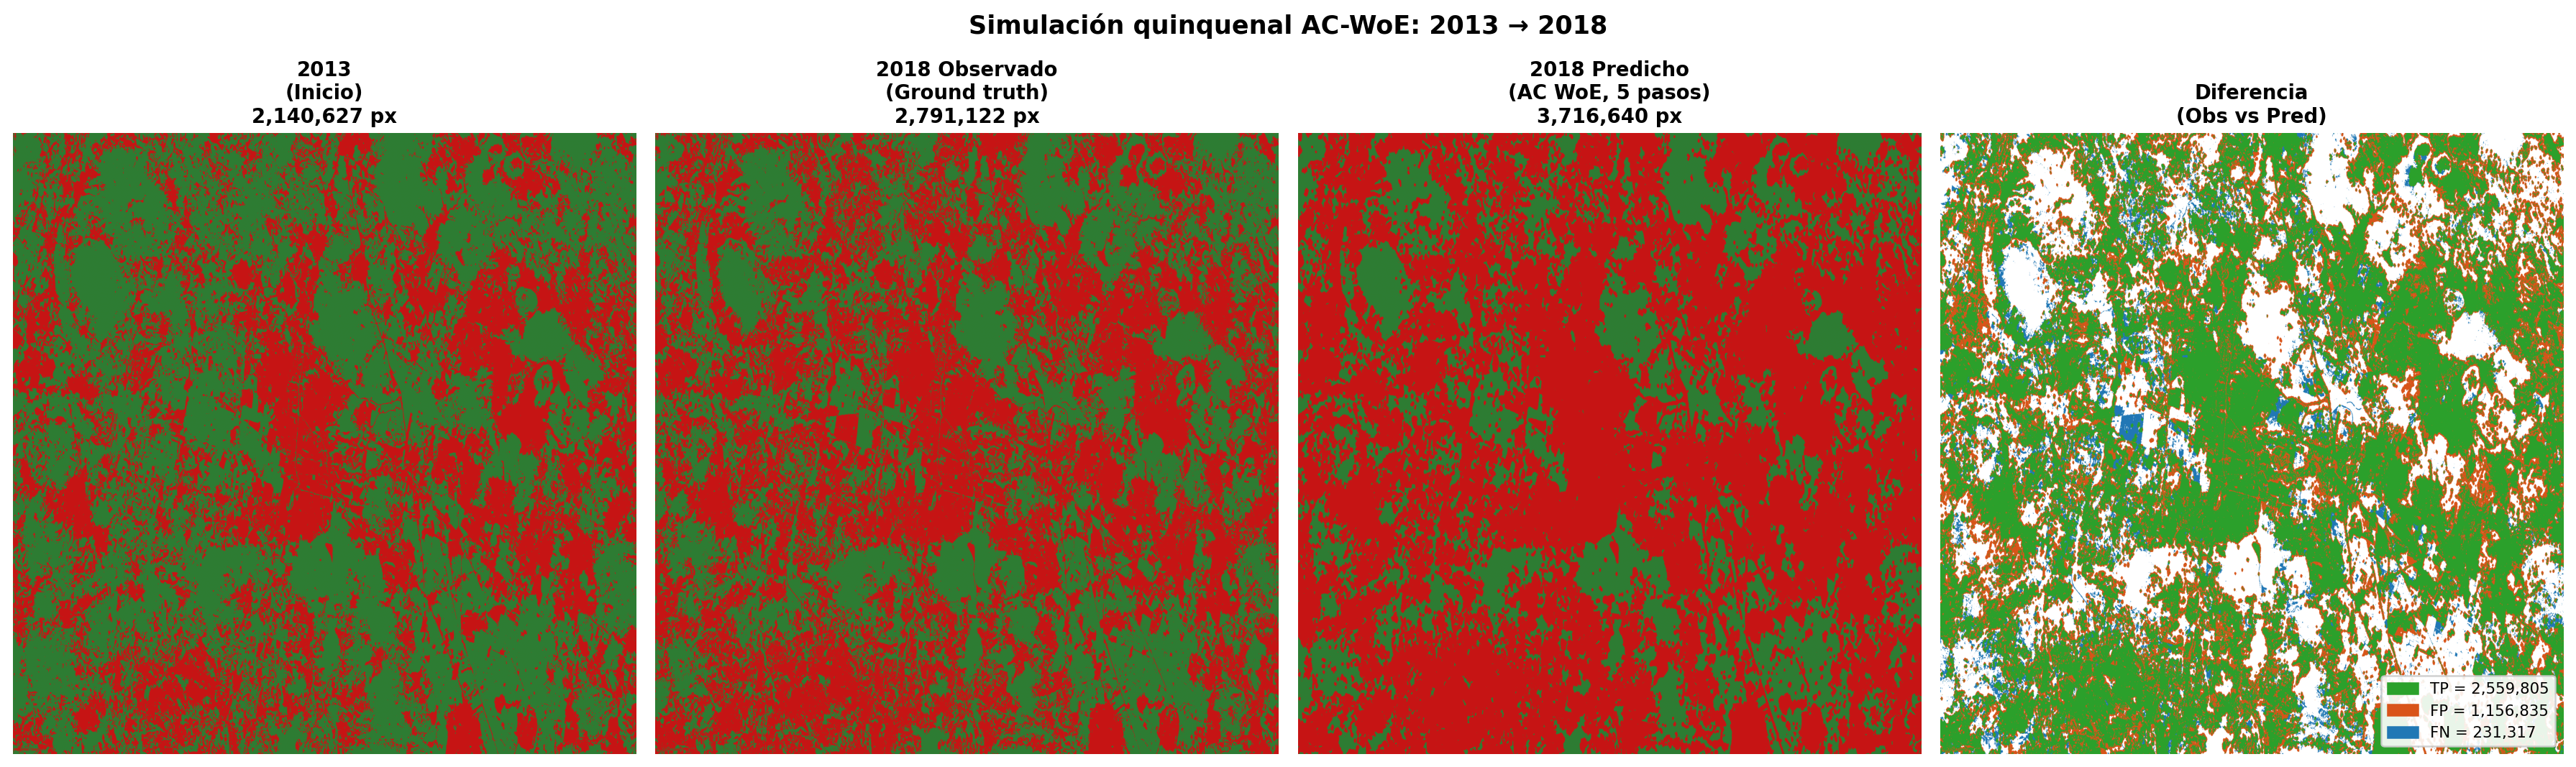
\includegraphics[width=\textwidth]{figures/summary_2013_to_2018.png}
\caption{Validación quinquenal 2013--2018. FoM $=0{,}355$; valor cercano al del período 2012--2017 en un contexto análogo de crecimiento observado positivo. El número de omisiones ($231\,317$ píxeles) sugiere que parte de la expansión hacia el norte y el este no queda recogida en la predicción bajo este experimento.}
\label{fig:summary_2013_2018}
\end{figure}

\clearpage
\subsection{Período 2014--2019}

Este período se aparta de la tendencia: la Tabla~\ref{tab:metrics_2014_2019} registra un FoM de $0{,}287$ y la Figura~\ref{fig:summary_2014_2019} deja ver el desajuste entre un crecimiento real modesto y una predicción de expansión más amplia.

\begin{table}[H]
\centering
\caption{Métricas de validación del período 2014$\rightarrow$2019.}
\label{tab:metrics_2014_2019}
\small
\begin{tabular}{lrlr}
\toprule
\multicolumn{2}{c}{\textbf{Métricas de píxel}} & \multicolumn{2}{c}{\textbf{Figure of Merit}} \\
\midrule
Accuracy  & $0{,}697$ & FoM                  & \textbf{$0{,}287$} \\
IoU       & $0{,}614$ & Hits ($B$)           & $511\,475$ \\
Precision & $0{,}628$ & Falsas alarmas ($A$) & $1\,176\,288$ \\
Recall    & $0{,}965$ & Omisiones ($C$)      & $93\,486$ \\
F1        & $0{,}761$ & TP / FP / FN         & $2\,611\,594$ / $1\,545\,800$ / $93\,486$ \\
$\kappa$  & $0{,}396$ & Crec.\ obs.\ / pred.\ & $+9{,}5\%$ / $+68{,}3\%$ \\
\bottomrule
\end{tabular}
\end{table}

\begin{figure}[H]
\centering
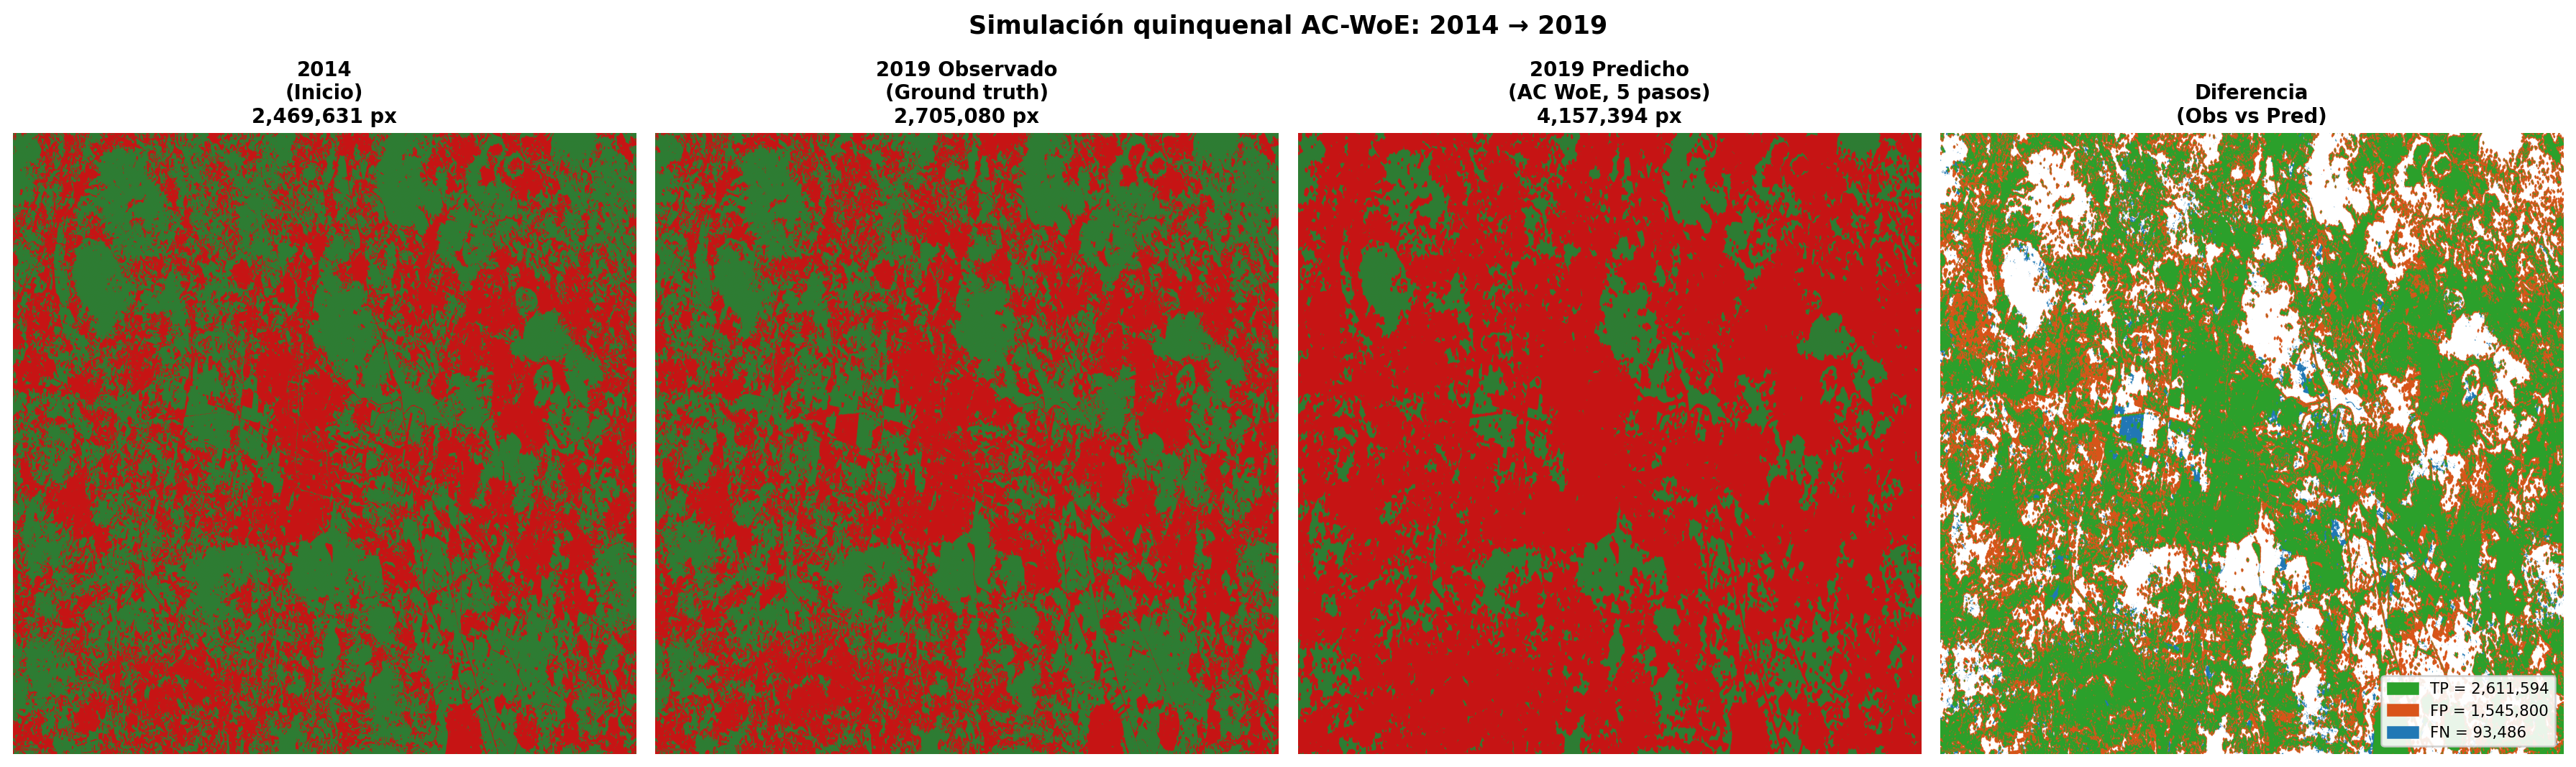
\includegraphics[width=\textwidth]{figures/summary_2014_to_2019.png}
\caption{Validación quinquenal 2014--2019. FoM $=0{,}287$; el crecimiento real modesto ($+9{,}5\%$) contrasta con una predicción de expansión más elevada ($+68{,}3\%$), lo que se refleja en la proporción de falsas alarmas ($1\,176\,288$ píxeles). El Recall alto ($0{,}965$) indica que el modelo asigna clase urbana de forma amplia respecto al mapa observado en 2019.}
\label{fig:summary_2014_2019}
\end{figure}

\clearpage
\subsection{Período 2015--2020}

La última ventana es la de FoM más alto de las cinco. La Tabla~\ref{tab:metrics_2015_2020} consigna un FoM de $0{,}378$ y la Figura~\ref{fig:summary_2015_2020} muestra el mayor número de aciertos de toda la serie, en un año de fuerte crecimiento observado.

\begin{table}[H]
\centering
\caption{Métricas de validación del período 2015$\rightarrow$2020.}
\label{tab:metrics_2015_2020}
\small
\begin{tabular}{lrlr}
\toprule
\multicolumn{2}{c}{\textbf{Métricas de píxel}} & \multicolumn{2}{c}{\textbf{Figure of Merit}} \\
\midrule
Accuracy  & $0{,}755$ & FoM                  & \textbf{$0{,}378$} \\
IoU       & $0{,}669$ & Hits ($B$)           & $704\,983$ \\
Precision & $0{,}701$ & Falsas alarmas ($A$) & $977\,214$ \\
Recall    & $0{,}936$ & Omisiones ($C$)      & $181\,887$ \\
F1        & $0{,}802$ & TP / FP / FN         & $2\,682\,235$ / $1\,145\,318$ / $181\,887$ \\
$\kappa$  & $0{,}498$ & Crec.\ obs.\ / pred.\ & $+33{,}5\%$ / $+78{,}4\%$ \\
\bottomrule
\end{tabular}
\end{table}

\begin{figure}[H]
\centering
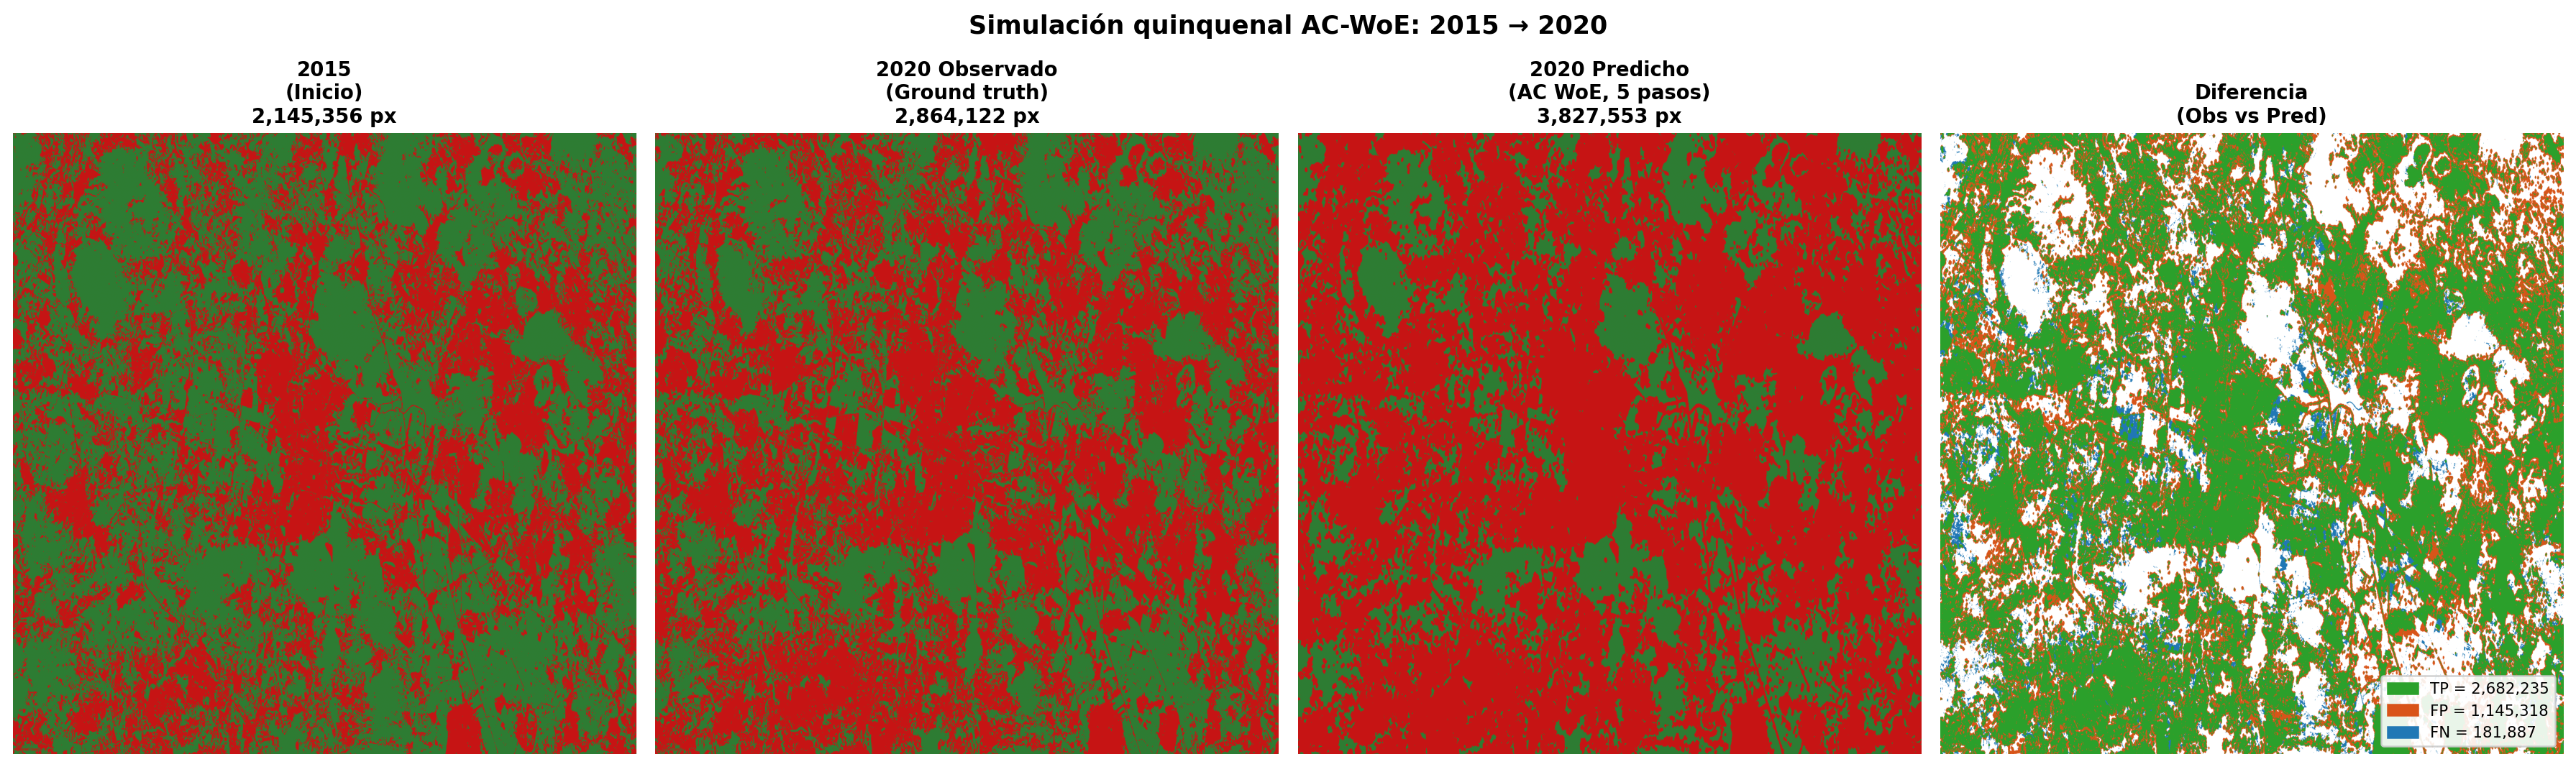
\includegraphics[width=\textwidth]{figures/summary_2015_to_2020.png}
\caption{Validación quinquenal 2015--2020. FoM $=0{,}378$; entre las cinco ventanas es el FoM más alto, en un contexto de fuerte crecimiento observado ($+33{,}5\%$). Se registran 704\,983 hits y, en términos relativos a este conjunto de corridas, una menor proporción de falsas alarmas que en otras ventanas.}
\label{fig:summary_2015_2020}
\end{figure}

\clearpage
% ============================================================
\subsection{Descomposición del desacuerdo en cantidad y asignación}
\label{sec:descomposicion-error}

Las métricas anteriores dicen cuánto se equivoca el modelo, no de qué se equivoca. La descomposición de \textcite{PontiusMillones2011}, definida en las ecuaciones~\ref{eq:desacuerdo_cantidad} y~\ref{eq:desacuerdo_asignacion} del marco teórico, separa las dos fuentes: predecir una extensión de cambio equivocada es desacuerdo de cantidad, y localizar mal un total correcto es desacuerdo de asignación. La Tabla~\ref{tab:pontius_decomposition} recoge ambos componentes en las cinco ventanas.

\begin{table}[htbp]
\centering
\caption{Descomposición del desacuerdo total en sus componentes de cantidad y de asignación \parencite{PontiusMillones2011}, sobre las $5\,419\,008$ celdas de cada ventana. El desacuerdo total es el complemento de la exactitud global de la Tabla~\ref{tab:metrics_all_periods}. La última columna es la fracción del desacuerdo atribuible a la cantidad.}
\label{tab:pontius_decomposition}
\begin{tabular}{lrrrr}
\toprule
\textbf{Período} & \textbf{FoM} & \textbf{Cantidad} & \textbf{Asignación} & \textbf{Cantidad / total} \\
\midrule
2011--2016 & $0{,}222$ & $31{,}1\%$ & $2{,}4\%$  & $92{,}9\%$ \\
2012--2017 & $0{,}345$ & $17{,}4\%$ & $7{,}6\%$  & $69{,}7\%$ \\
2013--2018 & $0{,}355$ & $17{,}1\%$ & $8{,}5\%$  & $66{,}7\%$ \\
2014--2019 & $0{,}287$ & $26{,}8\%$ & $3{,}5\%$  & $88{,}6\%$ \\
2015--2020 & $0{,}378$ & $17{,}8\%$ & $6{,}7\%$  & $72{,}6\%$ \\
\midrule
\textbf{Promedio} & $\mathbf{0{,}317}$ & $\mathbf{22{,}0\%}$ & $\mathbf{5{,}7\%}$ & $\mathbf{79{,}4\%}$ \\
\bottomrule
\end{tabular}
\end{table}

El desacuerdo de cantidad domina en las cinco ventanas y concentra el $79{,}4\%$ del desacuerdo total en promedio. El modelo urbaniza demasiadas celdas, pero las coloca en su mayoría donde corresponde. Ese diagnóstico es consistente con el Recall alto frente a la Precision moderada de la Tabla~\ref{tab:metrics_all_periods}, y con el factor de sobre-predicción que se documenta más adelante.

La lectura por ventana afina el resultado. Las dos ventanas de peor FoM son las de mayor desacuerdo de cantidad: 2011--2016 concentra en cantidad el $92{,}9\%$ de su desacuerdo, algo esperable porque es la única ventana con crecimiento neto observado negativo, de modo que cualquier crecimiento simulado es exceso por definición; en 2014--2019 la proporción llega al $88{,}6\%$. Las tres ventanas de mejor FoM descienden al rango $66{,}7$--$72{,}6\%$, y es ahí donde el desacuerdo de asignación alcanza su nivel más alto. La implicación metodológica es directa: el margen de mejora está en la estimación de la magnitud del crecimiento, no en la regla que decide dónde ocurre.

% ============================================================
\section{Análisis espacial del error del modelo}
% ============================================================

\begin{figure}[htbp]
  \centering
  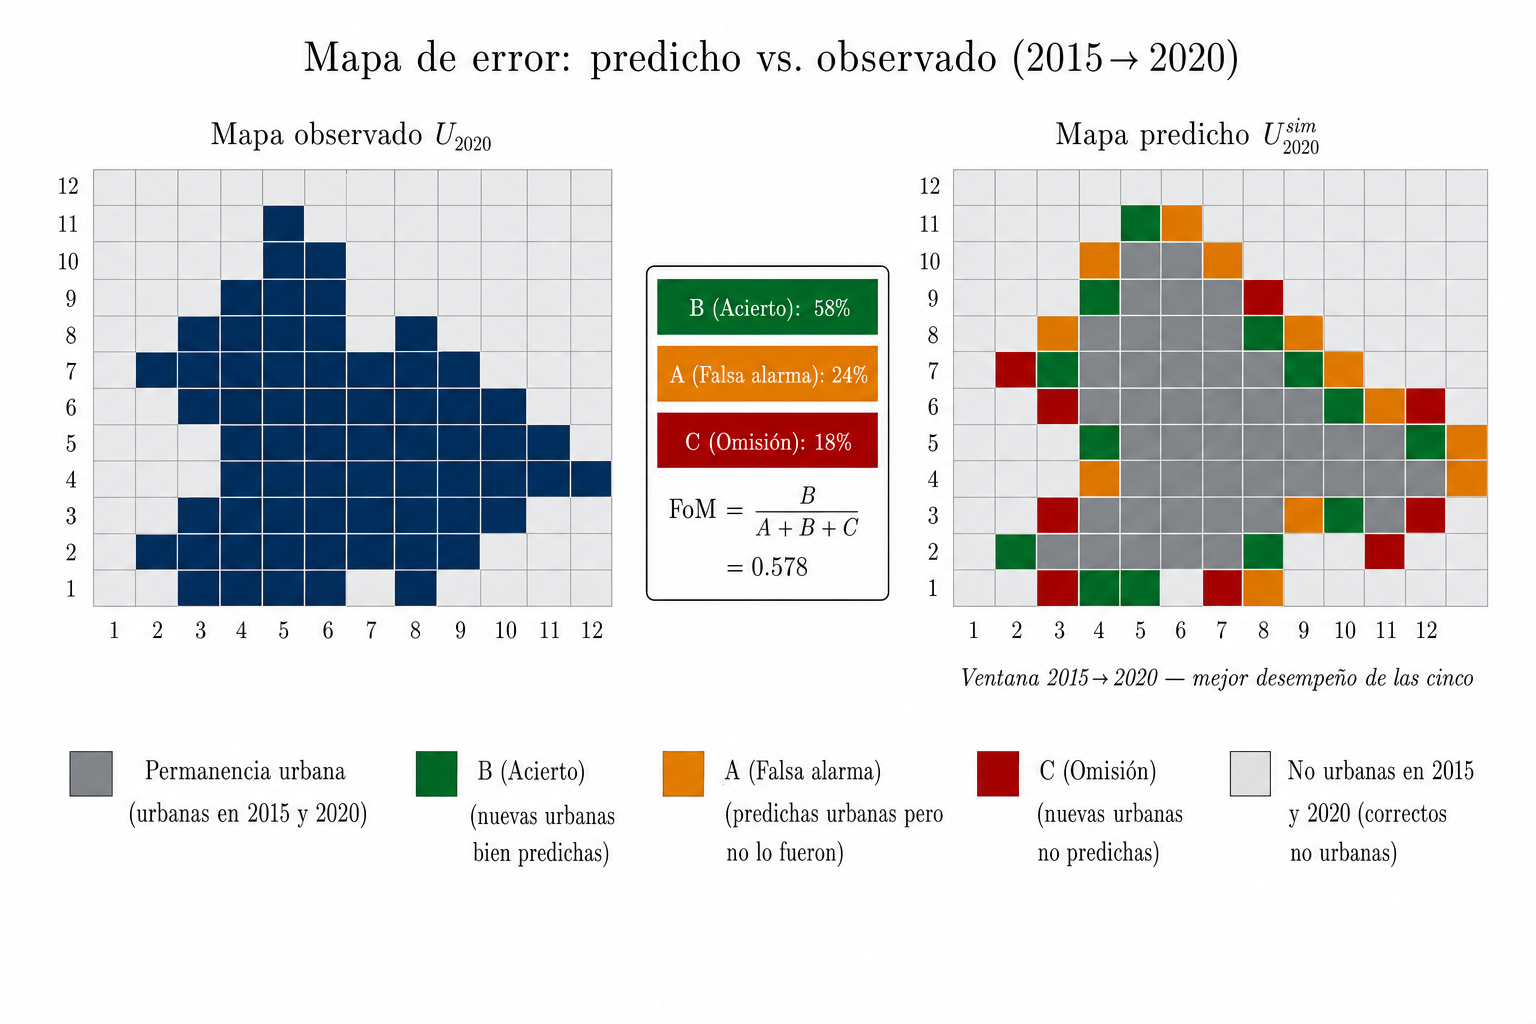
\includegraphics[width=0.90\linewidth]{F12_predicho_vs_observado_ai}
  \caption{Mapa de error para la ventana 2015$\rightarrow$2020 (FoM $=0{,}378$). Las celdas verdes (B) son aciertos, es decir, transiciones correctamente predichas; las ámbar (A) son falsas alarmas; las rojas (C) son omisiones. Solo las celdas en transición entran al cálculo del FoM; las permanencias urbanas y no urbanas aparecen en gris. \textit{Figura elaborada con IA generativa a partir de los mapas predicho y observado propios de la ventana 2015--2020.}}
  \label{fig:mapa-error}
\end{figure}

La Figura~\ref{fig:mapa-error} localiza esos componentes para la ventana 2015--2020. Complementando la evaluación cuantitativa, esta sección examina las fuentes de error identificadas en el proceso de simulación y analiza cualitativamente los patrones morfológicos de las predicciones, con el fin de orientar las extensiones metodológicas propuestas en las conclusiones.

\subsection{Fuentes de error identificadas}

El análisis conjunto de los cinco períodos revela tres fuentes principales de error que se propagan desde la clasificación de imágenes hasta la simulación:

\subsubsection{Error de clasificación de imágenes}

El pipeline de clasificación no supervisada (K-Means + SVM) reporta una concordancia interna de $88$--$94\%$ con las pseudoetiquetas en el conjunto de prueba holdout ($20\%$ de los píxeles), según se describe en el Capítulo~\ref{ch:modelo-crecimiento-urbano}. Con una imagen de $5{,}4$ millones de píxeles, un error nominal del $6$ al $12\%$ equivale a unos $325\,000$--$650\,000$ píxeles mal clasificados por imagen. Estos errores se manifiestan como confusión espectral (suelo desnudo o techos claros clasificados como urbano) e inconsistencias temporales que introducen ``transiciones'' espurias en el historial WoE.

\subsubsection{Propagación en transiciones históricas}

El cálculo de WoE se basa en las transiciones históricas observadas. Los errores de clasificación distorsionan las probabilidades WoE, y el efecto se acumula a lo largo de los 26 años de datos de entrenamiento.

\subsubsection{Amplificación en el autómata celular}

El AC amplifica errores iniciales: una celda mal clasificada como urbana actúa como ``semilla'' de crecimiento y genera falsas alarmas en cascada mediante el efecto de vecindad. La Tabla~\ref{tab:error_contribution} ordena estas tres fuentes por su contribución estimada, con la advertencia de que se trata de una estimación cualitativa y no de una descomposición medida.

\begin{table}[htbp]
\centering
\caption{Estimación cualitativa de la contribución de fuentes de error (no cuantificada empíricamente)}
\label{tab:error_contribution}
\begin{tabular}{lc}
\toprule
\textbf{Fuente de error} & \textbf{Contribución relativa estimada} \\
\midrule
Error de clasificación directa (K-Means+SVM) & Alta \\
Propagación de errores en el historial WoE & Moderada \\
Amplificación AC (efecto de vecindad cascada) & Alta \\
\bottomrule
\end{tabular}
\end{table}

\textbf{Nota metodológica:} la tabla anterior refleja una estimación \textit{cualitativa} basada en el análisis del comportamiento del modelo y no un desglose cuantificado de forma empírica. Una cuantificación precisa de la contribución de cada fuente de error requeriría mapas de referencia externos (verdad terreno) para cada año, los cuales no están disponibles para la serie completa 1984--2020.

\subsection{Análisis morfológico de la predicción}

El análisis morfológico cualitativo de los mapas generados muestra que el modelo reproduce patrones estructurales del crecimiento urbano coherentes con el observado: la expansión se concentra en los bordes de áreas ya urbanizadas (mecanismo de difusión), con presencia de fragmentación periférica. El mapa predicho para 2020 tiene un número de celdas urbanizadas mayor al observado (sobre-predicción sistemática), pero la distribución espacial del crecimiento sigue el mismo patrón de contigüidad que el real.

El cálculo formal de métricas de paisaje (FRAGSTATS, Moran's I) requeriría la ejecución de análisis específicos sobre los mapas predicho y observado. Los archivos de mapa predicho están disponibles, por ejemplo, en \path{data/processed/validation_quinquenal_2015_2020_v3_weighted/predicted_2020.npy}, para verificación independiente.

Conviene señalar el límite de esta lectura: la evaluación de este trabajo es píxel a píxel sobre las transiciones, que es lo que mide el FoM y donde el promedio alcanzado es $0{,}317$. La similitud morfológica se aprecia de forma visual, sin una métrica de configuración espacial que la cuantifique, de modo que no compensa ni sustituye la concordancia píxel a píxel. Incorporar métricas de patrón de paisaje para medirla es una de las extensiones que se plantean en las conclusiones.

% ============================================================
\section{Fortalezas y debilidades del modelo}
% ============================================================

\subsection{Fortalezas identificadas}

El modelo exhibe consistencia espacial: las predicciones concentran el crecimiento en los bordes de las áreas urbanas existentes, de forma coherente con el patrón de difusión observado. Su FoM promedio de $0{,}317$ se interpreta frente al espectro multi-sitio documentado por \textcite{pontius2008comparing} (Capítulo~\ref{ch:estado-del-arte}). El Recall se mantiene superior a $0{,}91$ en todos los períodos, de modo que el modelo recoge la mayor parte de las transiciones observadas bajo la definición operativa de la clase urbana. A esa cobertura se suma su fidelidad morfológica: las comparaciones visuales entre mapas predichos y observados (figuras \texttt{summary\_XXXX\_to\_XXXX.png} de cada período) muestran que el crecimiento predicho se concentra consistentemente en los bordes del área urbana existente y reproduce el patrón de difusión contigua observado en los cinco períodos. El enfoque es, además, parsimonioso: siete variables espaciales derivadas del mapa binario --distancia a área urbana, densidades de vecindad 3$\times$3/5$\times$5/7$\times$7, fragmentación local, gradiente urbano y tamaño de \textit{cluster}-- bastan para alcanzar estas métricas sin recurrir a datos socioeconómicos externos.

\subsection{Debilidades identificadas}

Las debilidades parten de una sobre-predicción sistemática: en las cuatro ventanas con crecimiento neto positivo el crecimiento predicho supera al observado por un factor de entre $2{,}3$ y $7{,}2$ veces, y en 2011--2016 el crecimiento observado es negativo, de modo que el cociente no está definido. Asociada a ella, la \textit{Precision} se mantiene moderada, entre $0{,}59$ y $0{,}70$, lo que indica que muchas predicciones de transición son falsas alarmas. El crecimiento disperso queda sin modelar: el mecanismo de vecindad no captura el desarrollo tipo \textit{leapfrog}. A ello se añade el peso de las variables externas, pues la omisión de factores socioeconómicos o de infraestructura (p.\ ej.\ distancia a empleo, precio del suelo) limita la precisión más allá de las siete variables derivadas del mapa binario.

% ============================================================
\section{Validación de hipótesis}
% ============================================================

A continuación se contrastan la hipótesis general y las cuatro particulares enunciadas en el Capítulo~\ref{ch:introduccion} con la evidencia de las cinco ventanas. El cuadro resumen se presenta en el Capítulo~\ref{ch:conclusiones}.

\textbf{H1 (apoyada por la evidencia, con una salvedad).} La regla de transición WoE ponderada por Information Value produce un modelo auditable: la distancia al frente urbano y la densidad de vecindad concentran el mayor IV, por encima de fragmentación y gradiente. La Tabla~\ref{tab:iv_weights} lo sostiene: distancia $0{,}282$ y las tres densidades suman $0{,}782$ del peso normalizado; fragmentación y gradiente quedan por debajo. La salvedad es la de la Sección~\ref{ssec:alcance-iv} y afecta al orden entre las dos primeras variables, no al enunciado: la primacía de la distancia sobre la densidad depende de un \textit{bin} sin transiciones observadas que, por construcción, ninguna celda candidata puede alcanzar. Lo que la hipótesis afirma queda en pie en cualquiera de las dos lecturas: la difusión por contigüidad gobierna la simulación y cada peso admite lectura geográfica, que es el sentido en que el modelo es auditable. Que la salvedad pueda enunciarse y cuantificarse con esta precisión es, de hecho, una consecuencia de esa auditabilidad.

\textbf{H2 (apoyada de forma parcial).} El desempeño se sostiene en las cinco ventanas desplazadas, pero el FoM varía entre $0{,}222$ y $0{,}378$ (Tabla~\ref{tab:metrics_all_periods}). El valor mínimo (2011--2016) coincide con la única ventana cuyo crecimiento neto observado es negativo. El comportamiento morfológico (expansión perimetral) se reproduce en todas las ventanas; las métricas píxel a píxel sí dependen de la señal de cambio. No hay degradación sistemática atribuible a un fallo de calibración, pero tampoco una estabilidad numérica estricta.

\textbf{H3 (apoyada por la evidencia).} El flujo completo se ejecutó en Python (NumPy, SciPy, scikit-learn) sobre capturas de Google Earth en escritorio, sin GPU ni software propietario, en un cómputo del orden de tres horas en CPU estándar.

\textbf{H4 (apoyada por la evidencia).} El FoM promedio de $0{,}317$, el Kappa de $0{,}445$ y el IoU de $0{,}633$ se ubican en la banda intermedia del espectro multi-sitio de \textcite{pontius2008comparing}, en los términos precisados en la Sección~\ref{sec:evaluacion}. El contraste con modelos de caja negra es cualitativo: sitios, clases y horizontes distintos.

% ============================================================
\section{Síntesis del desempeño del modelo}
% ============================================================
\label{sec:sintesis-desempeno}

Vistas en conjunto, las cinco ventanas dibujan un comportamiento consistente más que un resultado aislado. El FoM se mantiene en una banda intermedia (promedio $0{,}317$, entre $0{,}222$ y $0{,}378$) y el Recall alto en todos los períodos indica que el modelo rara vez deja fuera la urbanización que sí ocurre. El costo de esa cobertura es una sobre-predicción sistemática: el crecimiento simulado supera al observado y la \textit{Precision} se queda en un rango moderado. En otras palabras, el modelo opera en un régimen de alta cobertura predictiva y baja especificidad relativa: acierta dónde crece la ciudad, pero tiende a hacerla crecer de más. Este comportamiento es propagación conservadora en términos de omisión y expansiva en términos de falsos positivos, consecuencia de un campo de probabilidad WoE que favorece la expansión continua del estado urbano ante vecindades parcialmente urbanizadas.

Ese patrón es coherente con la lectura de los pesos WoE. La distancia al área urbana y la densidad de vecindad concentran $78{,}2$\% del \textit{Information Value}, de modo que la señal que gobierna la simulación es la difusión por contigüidad. Ahí está, a la vez, la fortaleza y el límite del enfoque: como es un modelo de caja blanca, se puede leer qué lo mueve; pero al apoyarse solo en variables derivadas del propio mapa binario, no captura el desarrollo disperso ni los factores socioeconómicos que explican parte del crecimiento real. La validación multi-período, más que un número único, es lo que da solidez a esta lectura, porque muestra que el comportamiento se sostiene bajo distintas dinámicas observadas. Las cinco corridas concentran el crecimiento en los mismos núcleos urbanos consolidados y corredores, de modo que el patrón espacial predicho depende sobre todo del estado inicial de cada ventana. Conviene precisar el alcance de esa observación: es una regularidad de las cinco simulaciones, no un resultado de convergencia, porque este trabajo no analizó el comportamiento asintótico del autómata ni su sensibilidad al estado inicial.

Estos resultados son el insumo del capítulo siguiente, donde se consolidan las hipótesis en un cuadro único, se precisan las contribuciones del trabajo y se discuten las líneas para corregir las debilidades aquí identificadas, en particular la sobre-predicción y el crecimiento tipo \textit{leapfrog}.
